\thispagestyle{plain}
\chapter{Evaluation}\label{sec:evaluation}

This chapter covers the experiments we conducted to understand our partitioning algorithms and then compare our partition-based index to state-of-the-art index structures. We will briefly go over the setup and the software parameters that were used for the experiments in \Cref{sec:setup}. Then we cover the datasets and workloads on which the experiments were evaluated in \Cref{sec:datasets}. Finally, we present the results of the partitioning algorithms and benchmarks in \Cref{sec:respartitions} and \Cref{sec:resperformance}.

\section{Setup}\label{sec:setup}
All benchmarking experiments were conducted on a machine with NUMA architecture and two \textit{Intel Xeon X5690} processors with a base frequency of 3.47 GHz and 190 GB of RAM. The operating system was \textit{Arch Linux} with a kernel version \textit{linux 5.18.12}. For the compilation of the benchmarking, we used \textit{clang++ 14.0.6} with the release optimization level 3 (using the \verb|-O3| flag).

The implementation for our B$^+$-tree is the \textsc{TLX btree\_map} for the TLX B-tree by \citeauthor{TLX} \cite{TLX}. The ART implementation is the \textsc{ARTPrimaryLB} from \citeauthor{sosd-vldb} \cite{sosd-vldb} because of its support for lower bound queries. Concerning the PGM index, we chose to use the standard variant provided by \citeauthor{Ferragina:2020pgm} \cite{Ferragina:2020pgm}, the \textsc{PGMIndex}. As index configuration parameters, we chose an inner slot size of 16 and a leaf slot size of 32 for the TLX B-tree. For our index, we chose the same inner slot size for a better comparison. Our index does not require a leaf slot size since we have variable-length leaf nodes where the size is determined by the partitioning algorithms. The error parameter of the PGM index was set to $\epsilon = 128$.

\section{Datasets and Workloads}\label{sec:datasets}

To evaluate our partitioning algorithms, we looked at a variety of datasets and workloads to get a good understanding of how our partitioning algorithms work in practice. As for the datasets, we used synthetic and real-world representatives first to see how the algorithms perform on pure datasets with a clear distribution and then see if the algorithms translate well to irregular patterns in real-world data. The following real-world datasets are taken from \citeauthor{Kipf2019} \cite{Kipf2019}. All datasets consist of 64-bit unsigned integers.

\Cref{fig:cdfs} shows the cumulative distribution function (CDF) of the keys in different datasets that were used throughout the experiments. In the top row, the left graph shows the CDF of dense, uniformly distributed keys from 0 to 100 million. Naturally, it corresponds to a simple linear function. The middle graph displays the same for the real-world \verb|osm| dataset. We can see that there are many keys located around $0.5 \cdot 10^{19}$ and $1.0 \cdot 10^{19}$, which corresponds to the jumps at these points in the CDF. The third CDF shows the distribution of the real-world \verb|fb| dataset. The particular shape of the CDF here is caused by large outliers in the key domain. In the second row, we see CDF of the real-world datasets \verb|books| and \verb|wiki|. \verb|osm| contains uniformly sampled OpenStreetMap locations represented by their Cell IDs, \verb|fb| is a version of a Facebook user ID dataset, \verb|books| is a dataset of book sale popularity, and \verb|wiki| contains Wikipedia article edit timestamps. Each of them consists of 200 million keys.

\begin{figure}
    \centering
    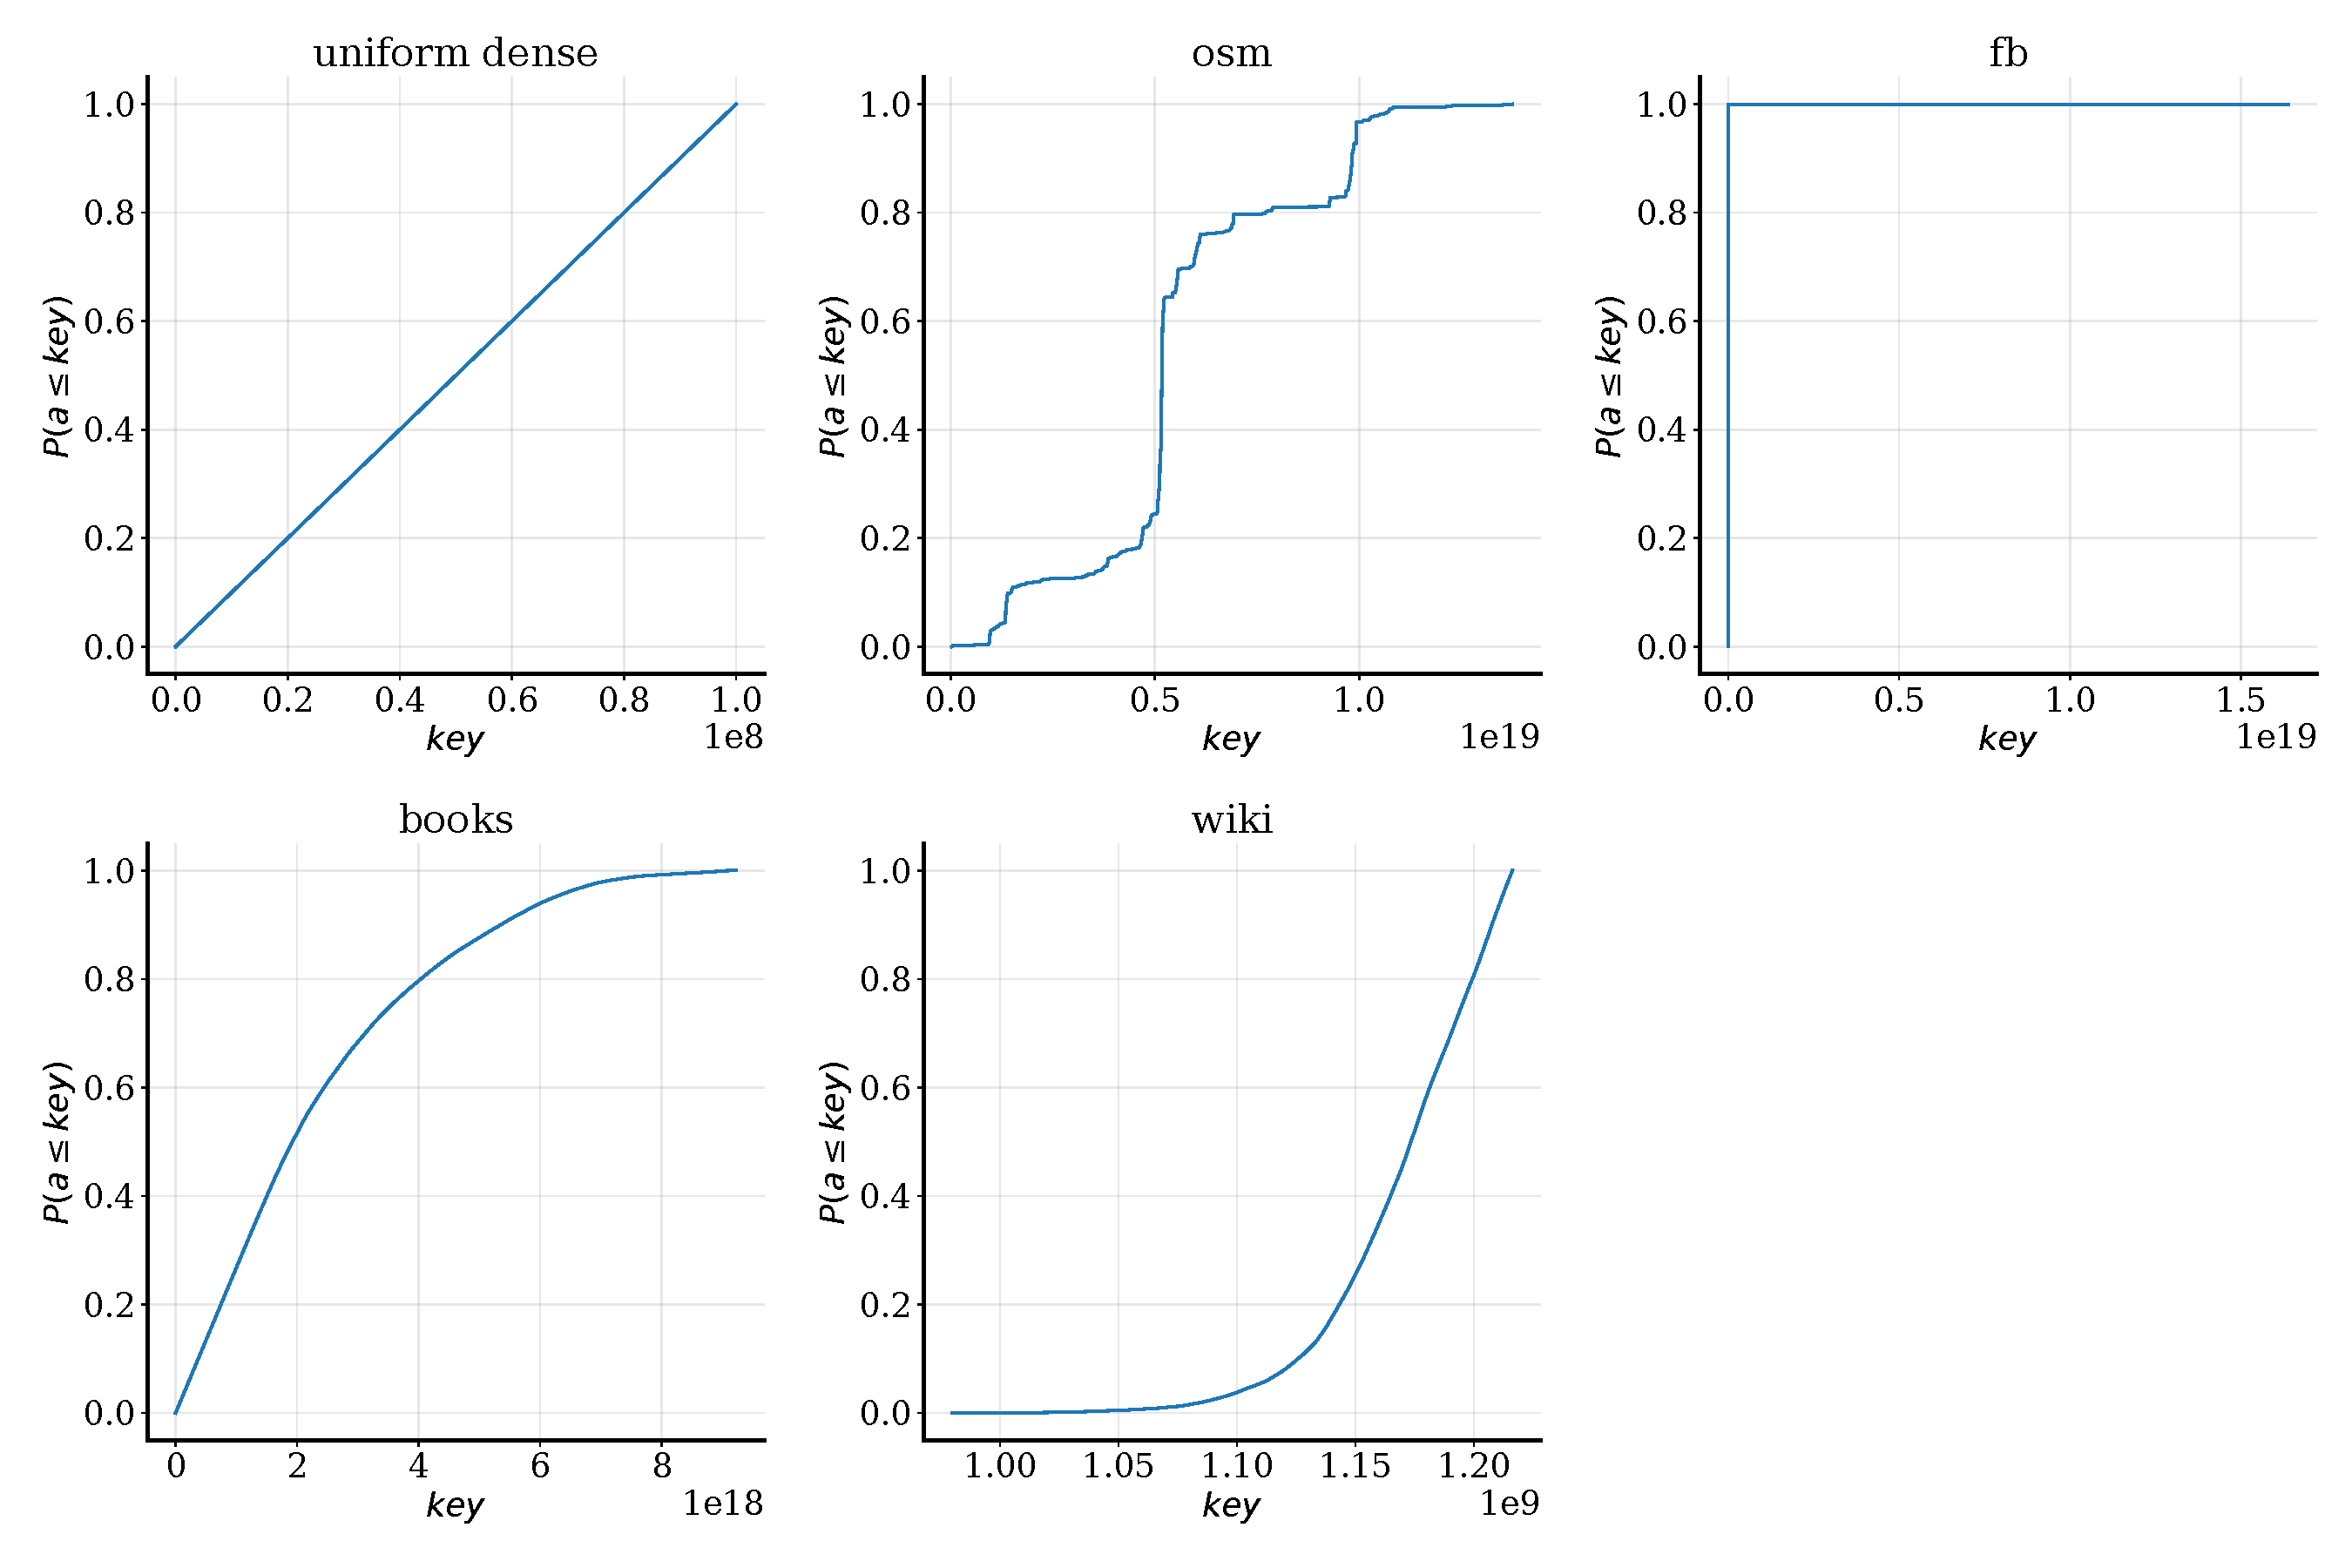
\includegraphics[width=\textwidth]{figures/cdfs.pdf}
    \caption{Cumulative distribution functions (CDF) of different datasets}
    \label{fig:cdfs}
\end{figure}

For the workloads, we proceed according to the generation described in \Cref{sec:wklgeneration}. Our workloads are generated using multiple \verb|Region| objects, where each can specify a distribution from which the queries should be sampled. For the sampling, we used \textit{Python 3.10.4} in combination with the \textit{scipy (1.7.3)} package. Before we describe the workloads in each experiment, we will now give a short overview of the fundamental distributions depicted in \Cref{fig:distributions}. 

The first distribution is a \verb|uniform| distribution. Its probability density function is given by

$$
f(x)=\begin{cases}
  \frac{1}{b - a} & \mathrm{for}\ a \le x \le b, \\[8pt]
  0 & \mathrm{for}\ x<a\ \mathrm{or}\ x>b
  \end{cases}
$$

\noindent The parameters $a$ and $b$ correspond to the region boundaries in our framework, which means that all the keys in a uniform region have the same probability of being sampled for our workload.

\noindent The second distribution is a \verb|normal| distribution, whose PDF is given by

$$
f(x) = \frac{1}{\sigma \sqrt{2 \pi}} \exp{(-\frac{1}{2}(\frac{x - \mu}{\sigma})^2)}
$$

\noindent The parameters $\mu$ and $\sigma$ regulate the location and scale of the PDF inside our region and represent the mean and standard deviation. The normal distribution is symmetric around $\mu$, which means that the keys around the center of the curve have the highest probability of being chosen for the workload, while the probabilities of the keys decrease symmetrically the further away they are from the center.

\noindent The third graph shows the PDF of a \verb|lognormal| distribution with its PDF used by \textit{scipy}

$$
f(x, s) = \frac{1}{s x \sqrt{2 \pi}} \exp{(-\frac{\ln{(x)}^2}{2 s^2})}
$$

\noindent According to their documentation, the location and scale parameters $\mu$ and $\sigma$ can be incorporated via the formula $f'(x, s, \mu, \sigma) = \frac{f((x - \mu)/ \sigma, s)}{\sigma}$. The parameter $s$ is also used influence the shape of the distribution. This distribution is highly skewed, which results in a non-symmetrical access pattern for the queries. 

\noindent Similarly, the last graph was created by a \verb|gamma| distribution. The \textit{scipy} documentation defines the PDF as 
$$
f(x, a) = \frac{x^{a - 1} e^{-x}}{\Gamma(a)}
$$

\noindent where we can again incorporate location and scale parameters $\mu$ and $\sigma$ using the conversion $f'(x, a, \mu, \sigma) = \frac{f((x - \mu)/ \sigma, a)}{\sigma}$. The parameter $a$ serves the purpose of changing the distributions shape. A gamma distribution is generally speaking very customizable when it comes to its shape, but for the sake of our purpose, we only choose the parameters such that we get a skewed distribution that is slightly less skewed than the lognormal distribution.

\begin{figure}
    \centering
    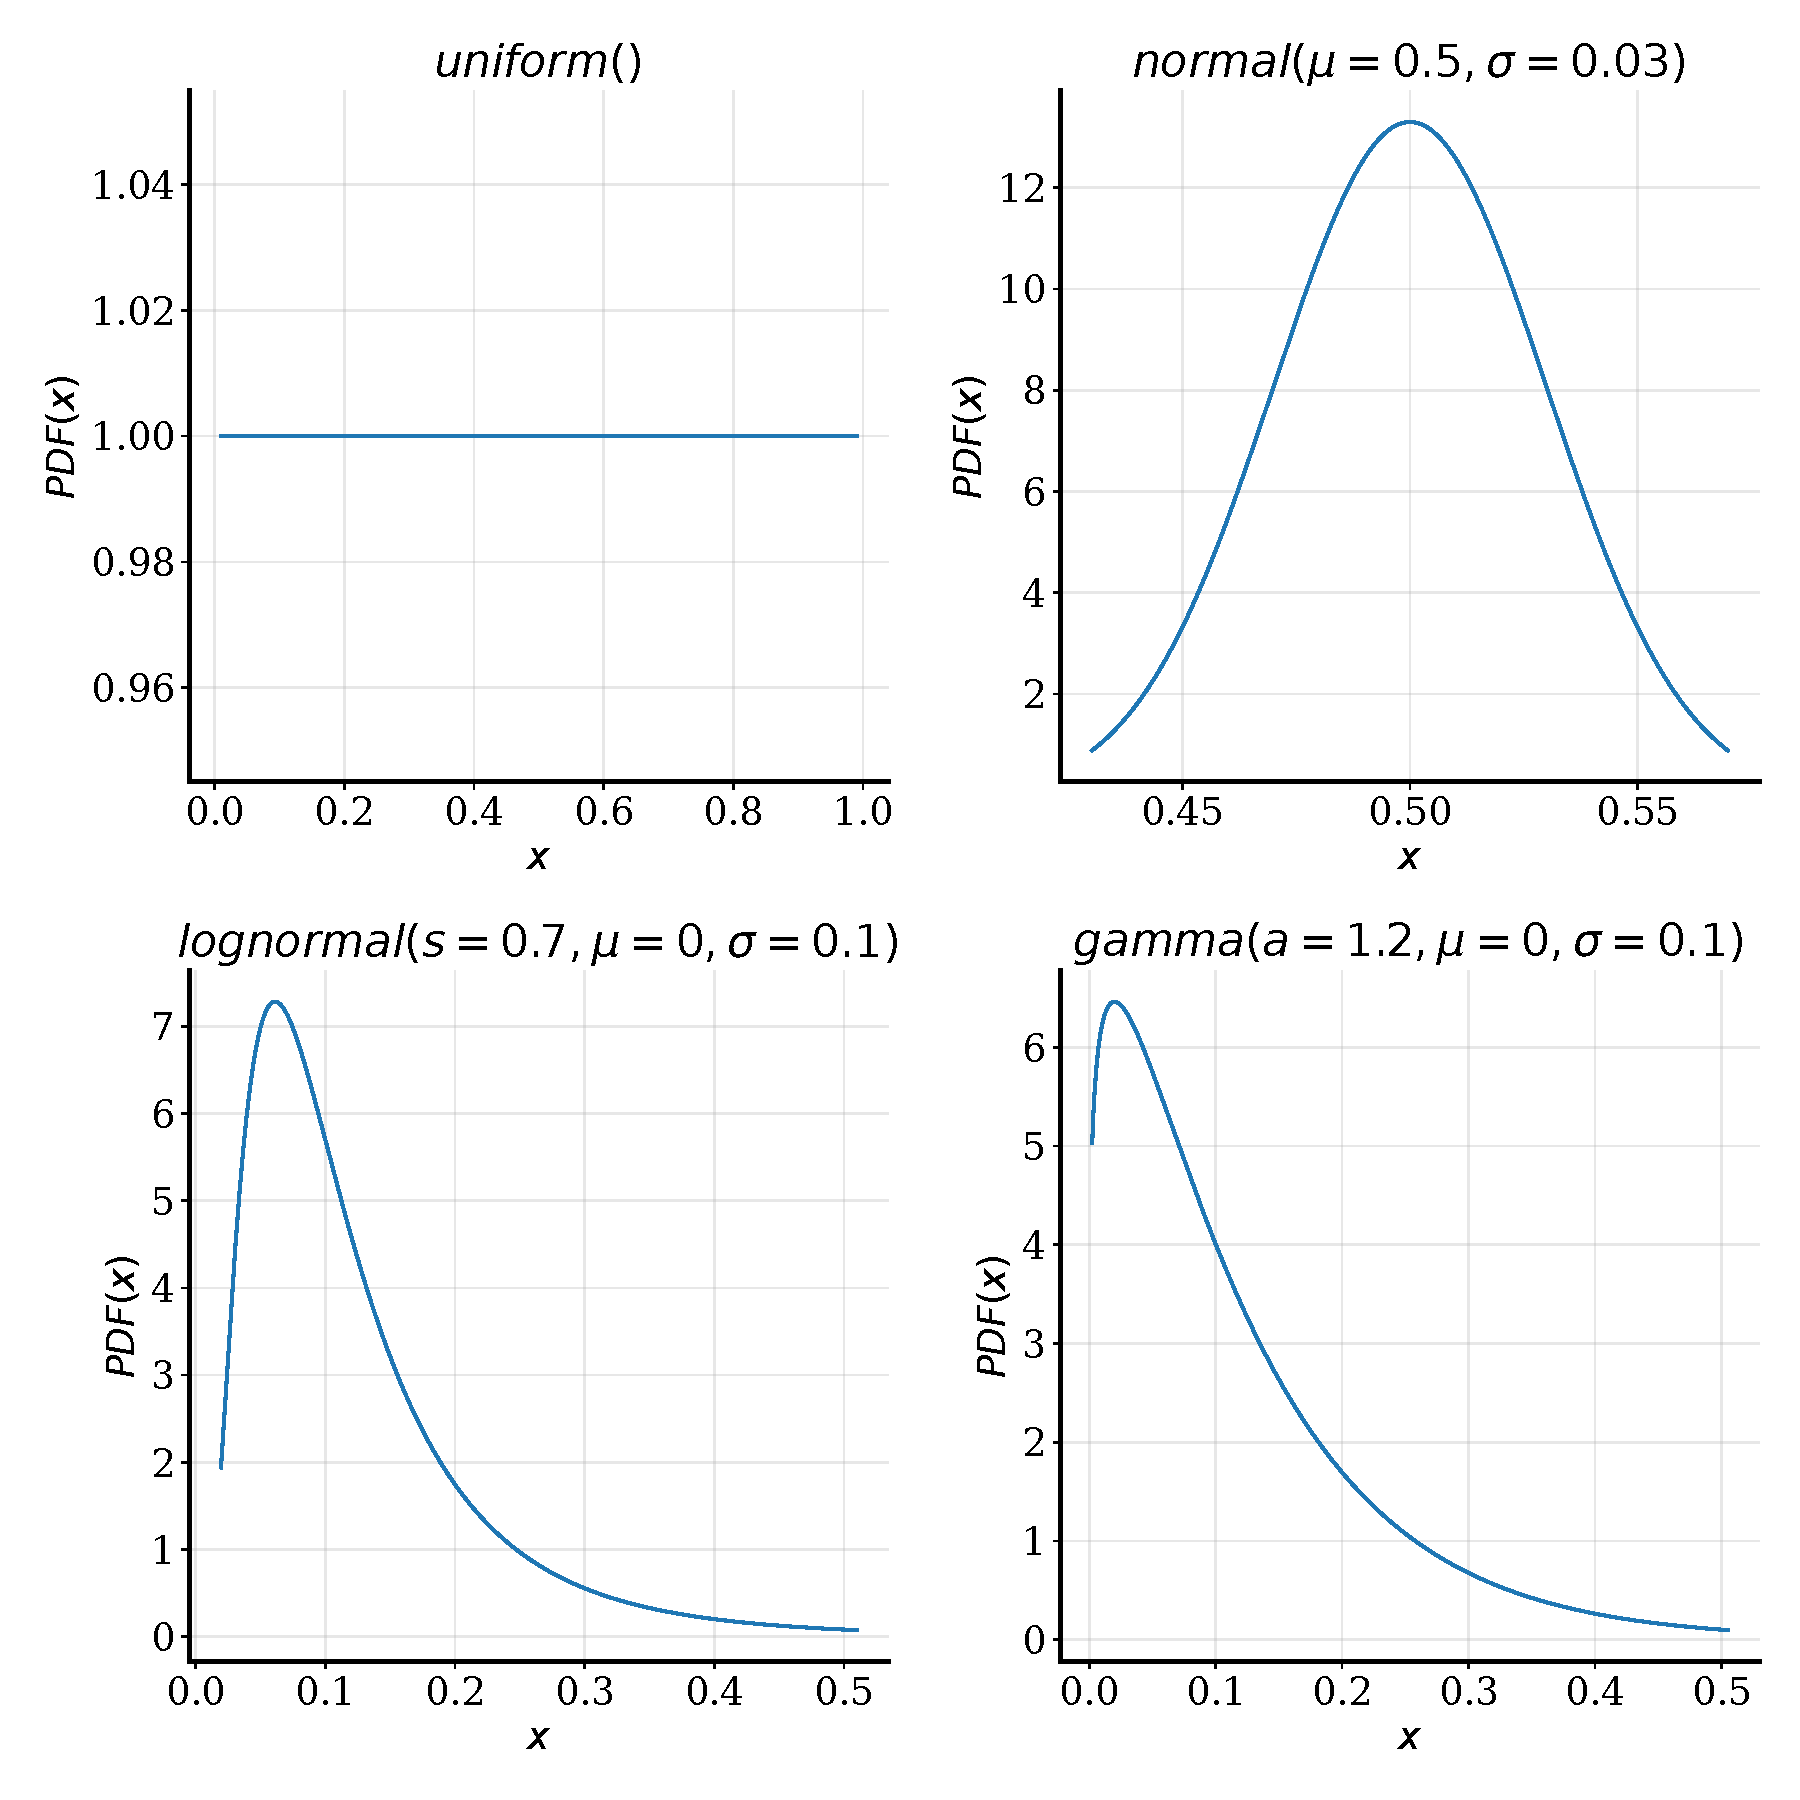
\includegraphics[width=\textwidth]{figures/distributions.pdf}
    \caption{Probability density functions (PDF) of different distributions}
    \label{fig:distributions}
\end{figure}

\section{Influence of Hyperparameters}\label{sec:respartitions}
Both our algorithms are based on a sliding window approach, so the hyperparameters to our partitioning naturally include the window size $w$. For the frequency approach, we also need to specify how lenient we want to be when determining whether a window is a plateau. As we will only seldom see that our frequency function is perfectly uniform in certain regions, we introduce the hyperparameter $\delta$. It gives us an upper bound for the absolute value of the discrete first-order derivative approximations over a window to allow classification as a plateau still. 

Although we have extensively varied these parameters throughout our experiments, we could not determine automatically what these parameters should be for a given dataset and workload. Only through manual inspection of the dataset and workload distribution could we choose an acceptable configuration such that the partitions intuitively fit the workload. This is easier for workload distributions like the uniform one, where we could directly adjust our window size $w$ and $\delta$ to translate the uniform region to a separate partition. However, for others, like the normal distribution, this is not as easy, as we cannot determine any obvious plateaus. Should we choose the parameters such that a region around the peak becomes its own partition? Should there be partitions around the tails of the distribution? What about the regions in between? These questions arise when there are no clear boundaries in our query distribution. Unfortunately, throughout our experiments, we could not find an answer that generalizes to all possible query distributions.

\subsection{Purity partitioning}
To showcase the behavior of the purity partitioning algorithm, we can look at the comparison depicted in \Cref{fig:purinfluence}. Both scenarios show the same query distribution, but on the left, we created partitions with the parameter $w = 200$, whereas on the right, we used $w = 1000$. The underlying data is a uniform, dense array of keys from 0 to 10,000. Over these 10,000 keys, we sampled uniformly 200,000 point queries each in the intervals [0, 3000) and [3300, 10000). In the remaining interval from [3000, 3300), we sampled uniformly 50,000 range queries. As the interval of range queries is only 300 keys long, the partitioning with $w = 1000$ will not recognize this region as a separate partition because at no point in this region will a sliding window of size 1000 produce a majority of range queries. Even in the middle of the range query region, at key 3150, the sliding window will only see 300 keys requested by range queries but 700 keys requested by point queries. Therefore, the whole key space is seen as a partition of mostly point queries. On the one hand, for $w = 200$, we can recognize that at key 3001, we have 99 point queries and 101 range queries in our window. Therefore, our algorithm will start a new partition at this index. On the other hand, as soon as we reach key 3301, we will see 99 range queries and 101 point queries, which will result in the start of yet another partition. As we can see, the window size selection plays a major role in whether regions of alternating query types can be identified. If we do not set this parameter appropriately, we might very well get subpar results for our partitioning.

\begin{figure}
    \centering
    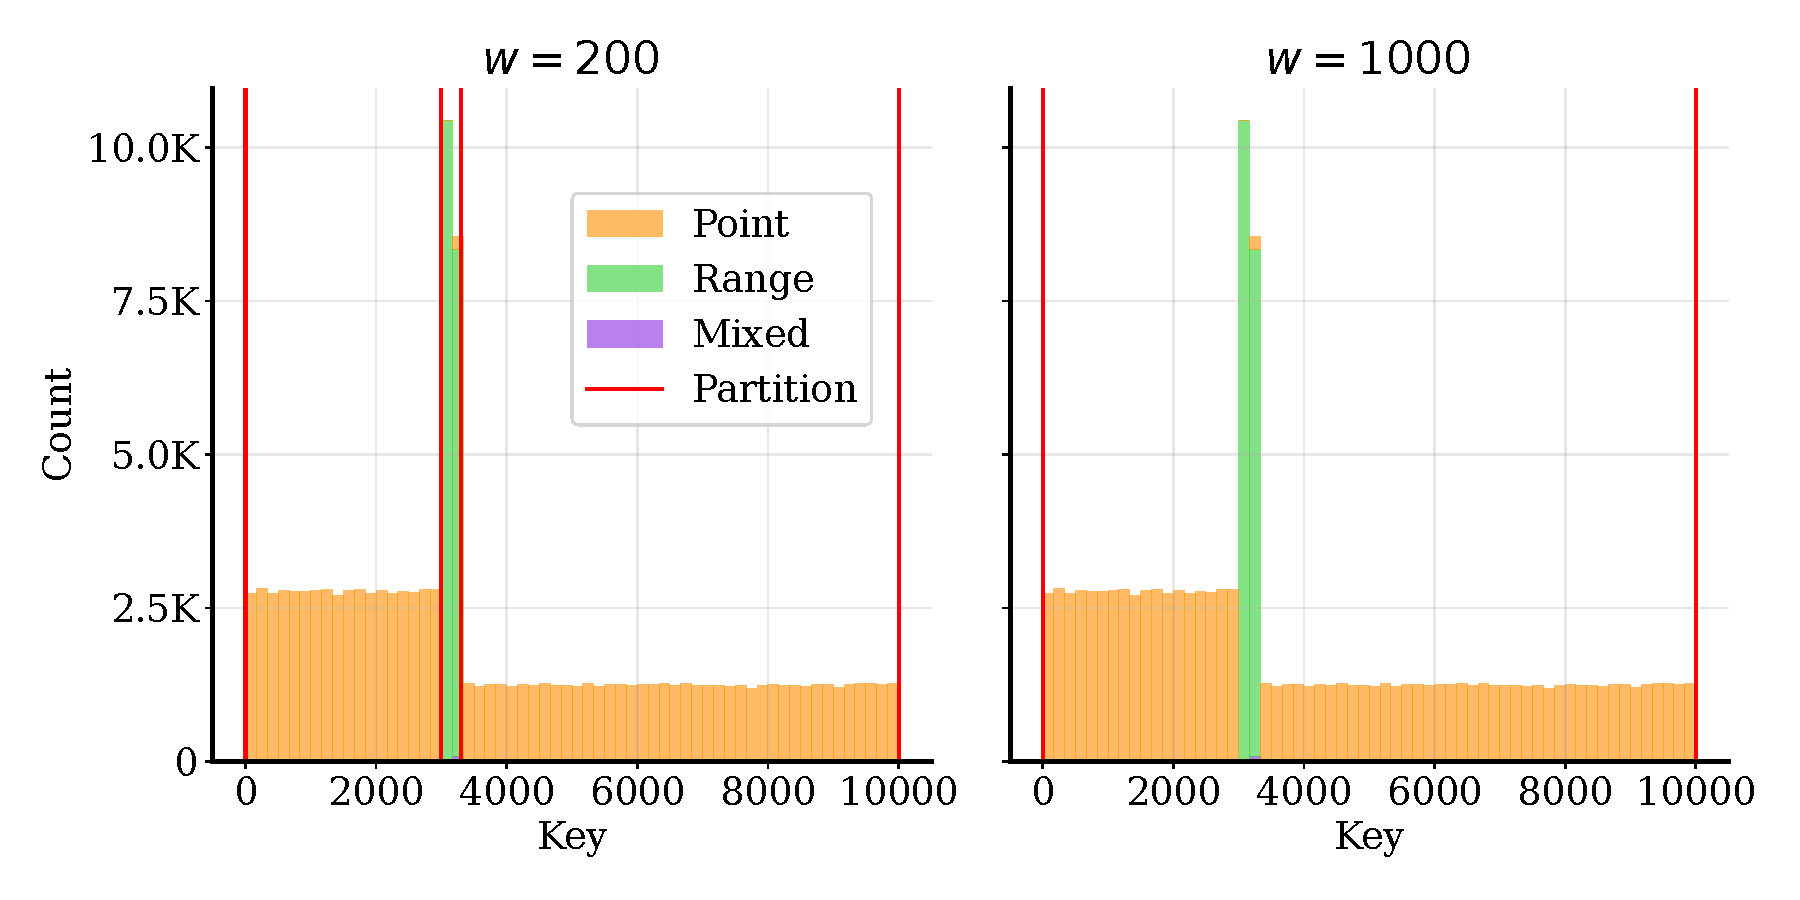
\includegraphics[width=\textwidth]{figures/purity_influence.pdf}
    \caption[Influence of purity hyperparameter]{Influence of window size parameter $w$ on purity partitioning. Left shows $w = 200$, right shows $w = 1000$.}
    \label{fig:purinfluence}
\end{figure}

\subsection{Frequency partitioning}
For our frequency approach, we have two parameters that need to be chosen beforehand. The first is identical to the purity approach presented in the last section, the window size $w$. The different finite difference approximations are then calculated over the frequencies in this window. A perfectly uniform region in the frequency domain would result in an approximation of zero. However, in practice, we will most likely see more variance in the frequency and also noise that does not follow a general pattern. Therefore, we do not get an optimal approximation of exactly zero, but something in its near vicinity. The parameter $\delta$ then influences whether this deviation from zero is small enough for it to be negligible. As an example, a configuration of the algorithm with window size $w = 100$ and $\delta = 3$ will allow a deviation of $\frac{\delta}{w} = \frac{3}{100} = 0.03$. For the forward approximation, this means that the frequency of the current key $f$ at index $i$ and the average frequency of the next 100 keys can differ by 3. The corresponding maximal slope $s$ is then identical to the previously introduced fraction $\frac{\delta}{w}$:

$$
s = \frac{\Delta y}{\Delta x} = \frac{(f + 3) - f}{(i + 100) - i} = \frac{3}{100} = \frac{\delta}{w}
$$

\noindent This relation is visualized in \Cref{fig:freqinfluence}. For the sake of simplicity, the workload represents a function with the following definition:

$$
f(x)=\begin{cases}
  40 & \mathrm{for}\ 3000 \leq x \leq 4000, \\[8pt]
  10 & \mathrm{for}\ x<3000\ \mathrm{or}\ x>4000
  \end{cases}
$$

\noindent where $f(x)$ evaluates to the access frequency of key $x$.

\noindent Note that this workload was not sampled using our framework. While our framework is very well able to do this generation, it inherently incorporates some variation in the steps due to the random nature of sampling. To showcase the influence of the parameters $w$ and $\delta$ however, we want to have a static frequency across each step with no variation.

\begin{figure}
    \centering
    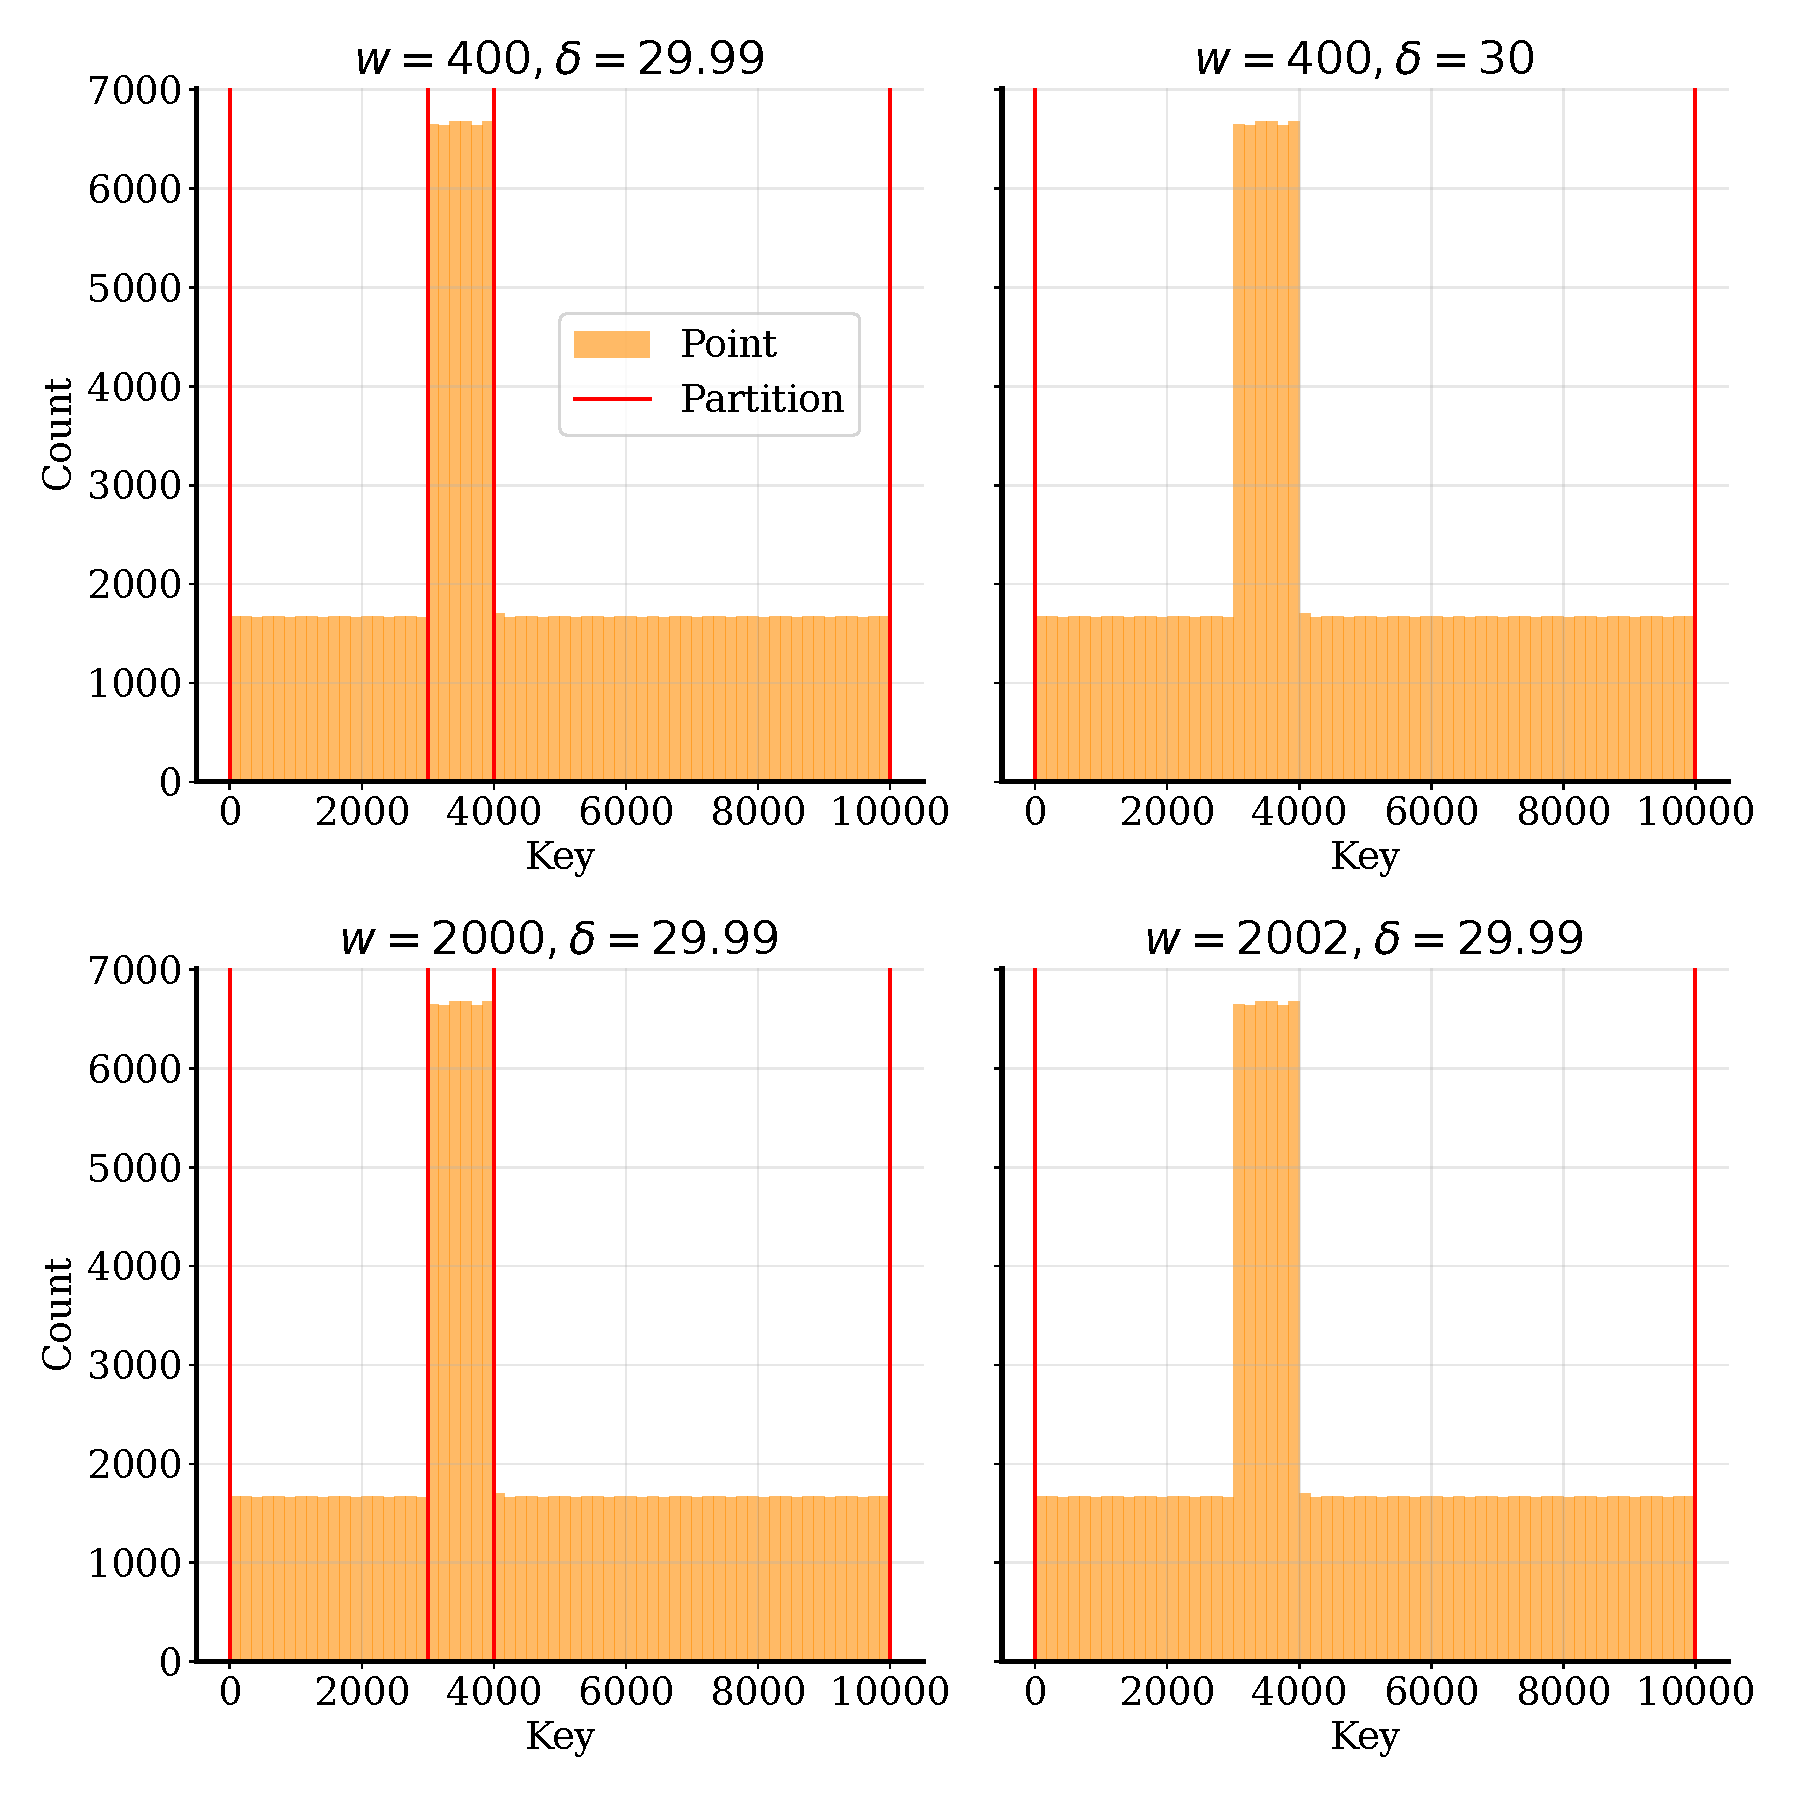
\includegraphics[width=\textwidth]{figures/freq_influence.pdf}
    \caption[Influence of frequency hyperparameters]{Influence of window size parameter $w$ and $\delta$ on frequency partitioning. The first row shows the influence of $\delta$ when the window size is fixed, and the second row shows the influence of $w$ when $\delta$ is fixed.}
    \label{fig:freqinfluence}
\end{figure}

The first two graphs show the influence of $\delta$ when the window size $w$ is fixed. For this we chose $w = 400$ and $\delta_1 = 29.99, \delta_2 = 30$. According to our algorithm, to conclude a partition, we need a point where the average frequency of the left 200 keys differs more than 29.99 (30) from the average frequency of the right 200 keys. If we now look at key 3000, we see that the left 200 keys have an average frequency of 10 and the right 200 keys have an average frequency of 40. The difference is therefore 30. As $30 > 29.99 = \delta_1$, our partitioning algorithm produces a new partition for the keys between 3000 and 4000. However, since 30 is not strictly greater than $\delta_2 = 30$, the algorithm produces no separate partition in the second case.

In the second row, we investigate the influence of $w$ when $\delta$ is fixed. We chose $\delta = 29.99$ and $w_1 = 2000, w_2 = 2002$. Again, to form a new partition, we need a point where the average frequency of the left 1000 (1001) keys differs more than 29.99 from the average frequency of the right 1000 (1001) keys. Let us now look again at key 3000. We can determine that the average frequency of the left 1000 and 1001 keys is 10. However, for the right keys, there is a difference. If we only look 1000 keys to the right, we exhaust the complete plateau of elevated frequencies. The average frequency is here 40. However, if we look 1001 keys to the right, we not only include all keys with frequency 40 but also one with frequency ten again. Therefore, the average frequency is $\frac{40 \cdot 1000 + 10}{1001} = 39.97$. The difference in average frequencies is 30 for the first case and 29.97 for the second. As our threshold is $\delta = 29.99$, the algorithm will only create a new partition in the first case, not in the second.


\section{Benchmarking results}\label{sec:resperformance}
After all indexes are constructed, we run the test workload ten times on each of them, shuffling after each run to prevent caching effects. We apply the same strategy as \citeauthor{Dittrich2021} when it comes to range queries, namely that they can be translated to a lower bound query and a subsequent scan of the data array. This is possible because our scenario is that index entries map keys to their position in a sorted array. The scan of the data array is independent of the index type and can be neglected. Furthermore, we remark that all lookup time charts have small black bars that indicate the standard deviation across ten runs. As these are barely noticeable, we conclude that our results are quite stable.

\subsection{Purity partitioning on sharp borders}
First of all, we conducted an experiment that was designed to confirm the results of \citeauthor{Dittrich2021} \cite[Optimized vs Heuristic Indexes]{Dittrich2021}. It serves to answer the question: 

\begin{center}
    \textit{Can we reproduce the results presented in their paper?}
\end{center}

\noindent While they handcrafted the boundaries, the partitions for the experiment here were generated by our purity partitioning algorithm. The workload that was executed on the data was split into three regions: the first 10 percent of the keys, the next 75 percent, and finally the remaining 15 percent. The first region received 20 percent of the total queries as point queries, the second region received 10 percent of the queries as point queries, and 20 percent as range queries. The final region received the remaining 50 percent of queries as point queries. For our experiment, we used 2 million queries in total of which 1 million served as a train workload and 1 million as a test workload. For the benchmarking on the test workload, we, therefore, had the queries depicted in \Cref{tab:poc_wkl}.

\begin{table}
\centering
\begin{tabular}{rrrrr}
\hline
Region & from & to   & number queries & query type \\ \hline
1      & 0    & 0.1  & 200k           & Point      \\
2      & 0.1  & 0.85 & 100k           & Point      \\
2      & 0.1  & 0.85 & 200k           & Range      \\
3      & 0.85 & 1    & 500k           & Point      \\ \hline
\end{tabular}
\caption{Query Distribution for our first experiment}
\label{tab:poc_wkl}
\end{table}

\begin{figure}
    \centering
    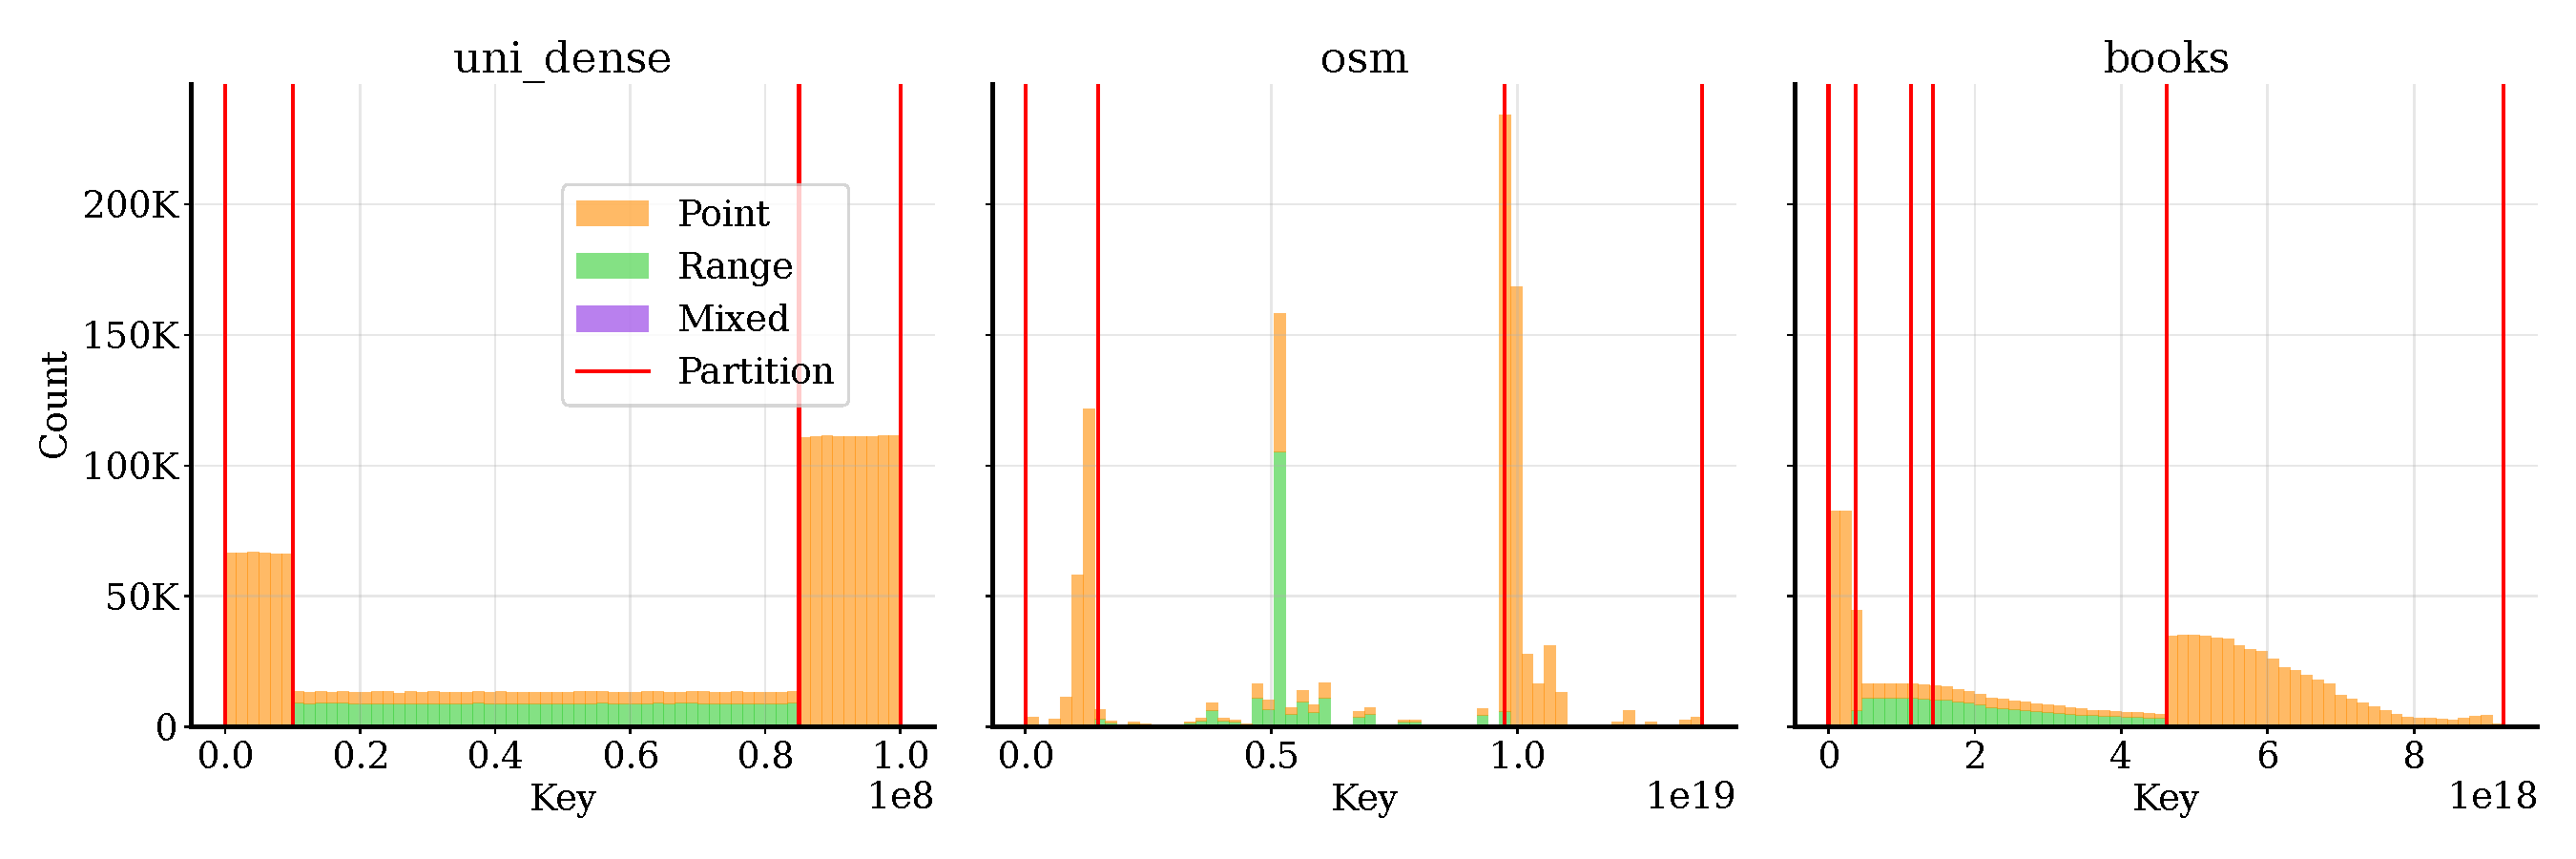
\includegraphics[width=\textwidth]{figures/exp1_query_dist.pdf}
    \caption[uniform, osm and books query distribution after sharp boundary sampling]{Query distribution in our first experiment, sampled over a uniform, dense dataset, the osm and the books dataset}
    \label{fig:poc_dist}
\end{figure}

The resulting query distribution, together with the boundaries that our algorithm produced, is visualized in \Cref{fig:poc_dist}. As we can already tell from the description of the query distribution, we have two very clear boundaries when looking at the purity. While the first and last regions are only requested by point queries, we can see that the middle part receives both types of queries. Notably, we see mostly orange and green bars in the figure in this region, as this range contains 150 million keys but receives only 300 thousand queries. While there is some overlap in these queries, it is rather unlikely that one key from this range is selected for both point and range queries. This overlap would result in a purple bar in the figure. Nevertheless, a generalizing partitioning algorithm should recognize the boundaries and create three partitions accordingly. 

The window size parameter $w$ was set to 10,000 because we know that the regions defined above contain multiple millions of keys. The resulting partitions reflect this anticipation. Only for the \verb|books| dataset do we see one additional partition in the middle of the mixed region. This extra partition is caused by the rare scenario we just described. While we have a region with mostly disjoint point and range queries, there are enough keys that are both requested by point and range queries. So our algorithm recognizes that the majority changes from range queries to mixed queries in our sliding window, creating this additional partition. We decided to include the same datasets here as \citeauthor{Dittrich2021}, but we also evaluated this workload on the remaining datasets \verb|fb| and \verb|wiki|. The corresponding plots can be found in \Cref{app:sharp}.

\Cref{fig:poc_times} shows the results of executing the test workload on the different data structures. AS we expect, our index consists of three leaf nodes, where the outermost contain a hast table and the middle one is a B-tree like leaf with sorted data. Depicted is the average lookup time for the 1 million queries. Across the three datasets, the TLX B-tree requires the most amount of time, between 700 and 800 ns. Both ART and PGM can outperform our index with lookup times around 120 ns for the uniform dense dataset. On the other two real-world datasets \verb|osm| and \verb|books|, our custom index achieves a competitive lookup time of around 250 ns, while ART and PGM require between 300 and 400 ns each. As \citeauthor{Dittrich2021} have also mentioned in their experiment, the uniform dense dataset is close to optimal for PGM and ART, which inherently puts our index at a disadvantage.  

\begin{figure}
    \centering
    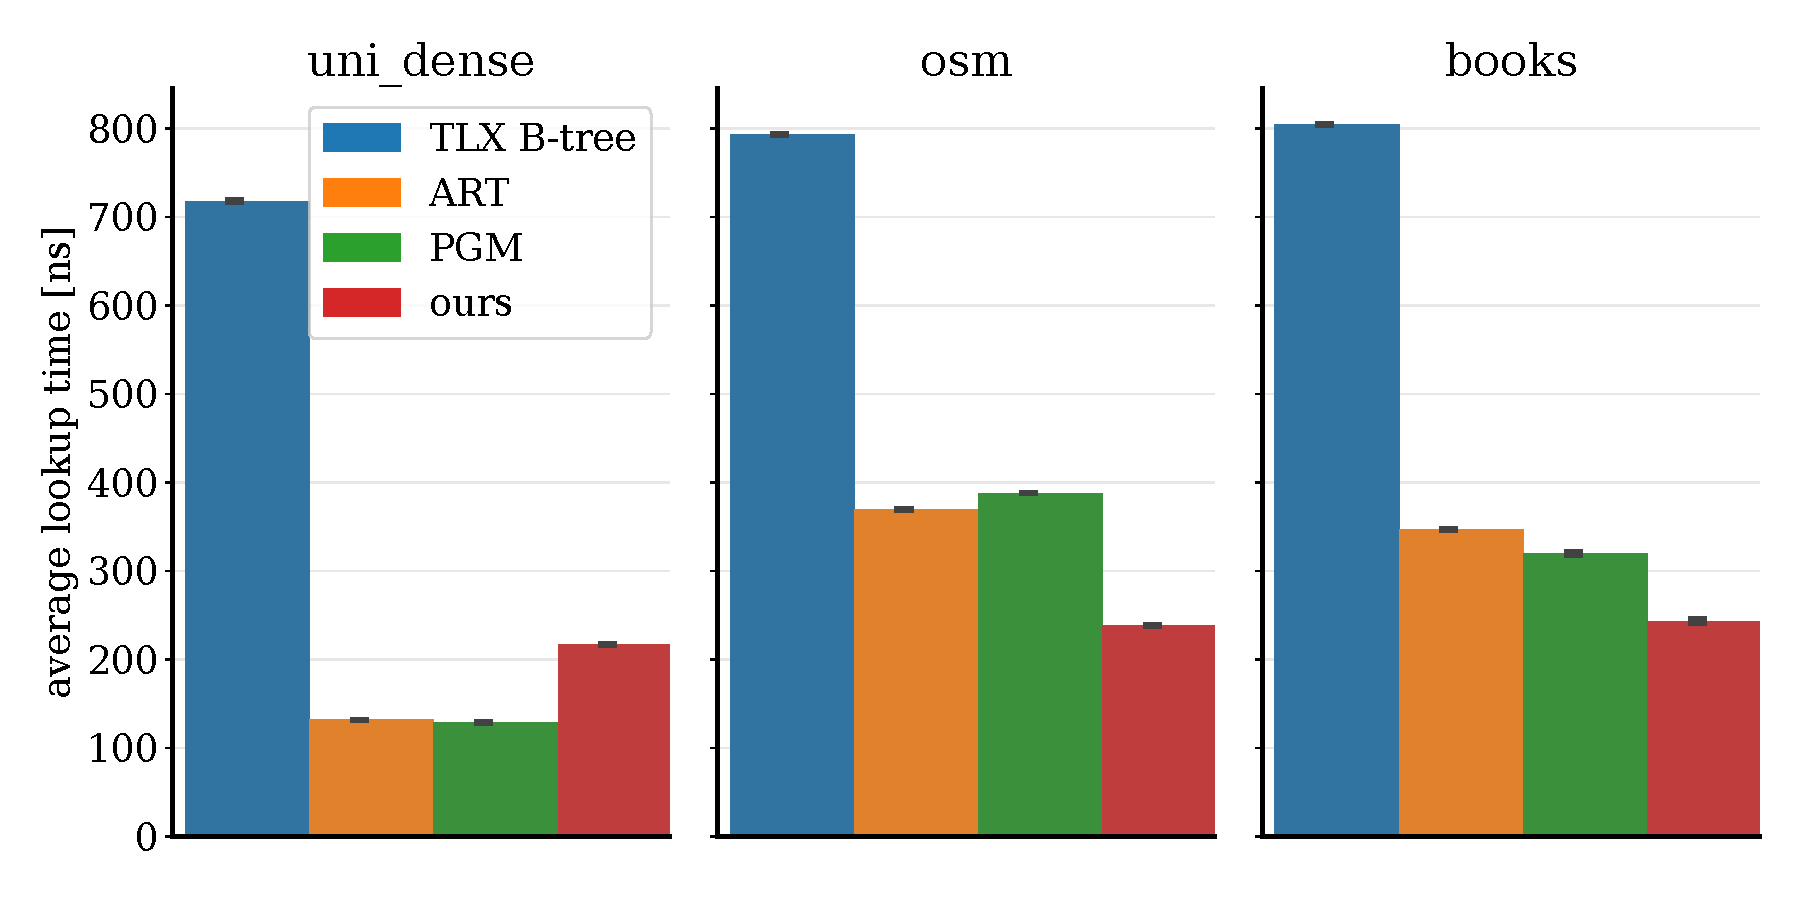
\includegraphics[width=0.9\textwidth]{figures/poc_times.pdf}
    \caption[uniform, osm and books lookup performance after sharp boundary sampling]{Average query lookup time on uniform, dense data, and the osm and books dataset}
    \label{fig:poc_times}
\end{figure}

To come back to our initial question, we conclude that when there are optimal preconditions (i.e.~sharp transitions between query types), it is indeed possible for our partitioning algorithms to produce partitions that can compete with the state-of-the-art indexes ART and PGM. However, this custom workload is very customized to create a best-case scenario for our algorithm, with clear boundaries between point and range queries. The next experiments will cover our partitioning algorithm's performance in less optimal but more realistic scenarios.

\subsection{Worst case considerations}
Following the previous optimal setting, we looked at scenarios that are the worst case for our partitioning algorithms. The question that we want to answer through this experiment is:

\begin{center}
    \textit{What is the performance of our workload-based partitioning in the worst case?}
\end{center}

\noindent We first look at the scenario that represents the worst case for our frequency algorithm. The first graph in \Cref{fig:freqworst} shows the uniform query distribution across a uniform dataset with 10 million keys. Since we have no variation across the whole dataset, our partitioning algorithm generates only one large partition. To achieve this result, a window size of $w = 200$ and $\delta = 1$ was already sufficient. We have decided to look at two extremes as the worst case for the purity algorithm. Here, 2 million point and range queries are distributed uniformly across the same uniform dense dataset. The first case uses a large window with window size $w = 1000$. This window is large enough to neglect the variation between keys that are requested by point and/or range queries. The second case happens when we choose a smaller window size of $w = 200$. Here, the sampling variance is large enough to continuously cause the algorithm to start new partitions because the majority of query type changes in the sliding window. Instead of one partition, we end here with nearly 10,000 partitions. That is why the third graph is seemingly completely red. There are just too many partitions to see the space in between. Notice that we reduced the dataset size from 100 million to 10 million points. This is due to the implementation of our frequency algorithm in \textit{Python}, which already took several minutes to run on the reduced dataset. While there are ways to optimize the run time, e.g.~not computing the mean of the window for every step of the sliding, instead keeping track of the contents of the window and only adding/removing at the start/end, we only found time to include this optimization in the simpler purity algorithm. 

\begin{figure}
    \centering
    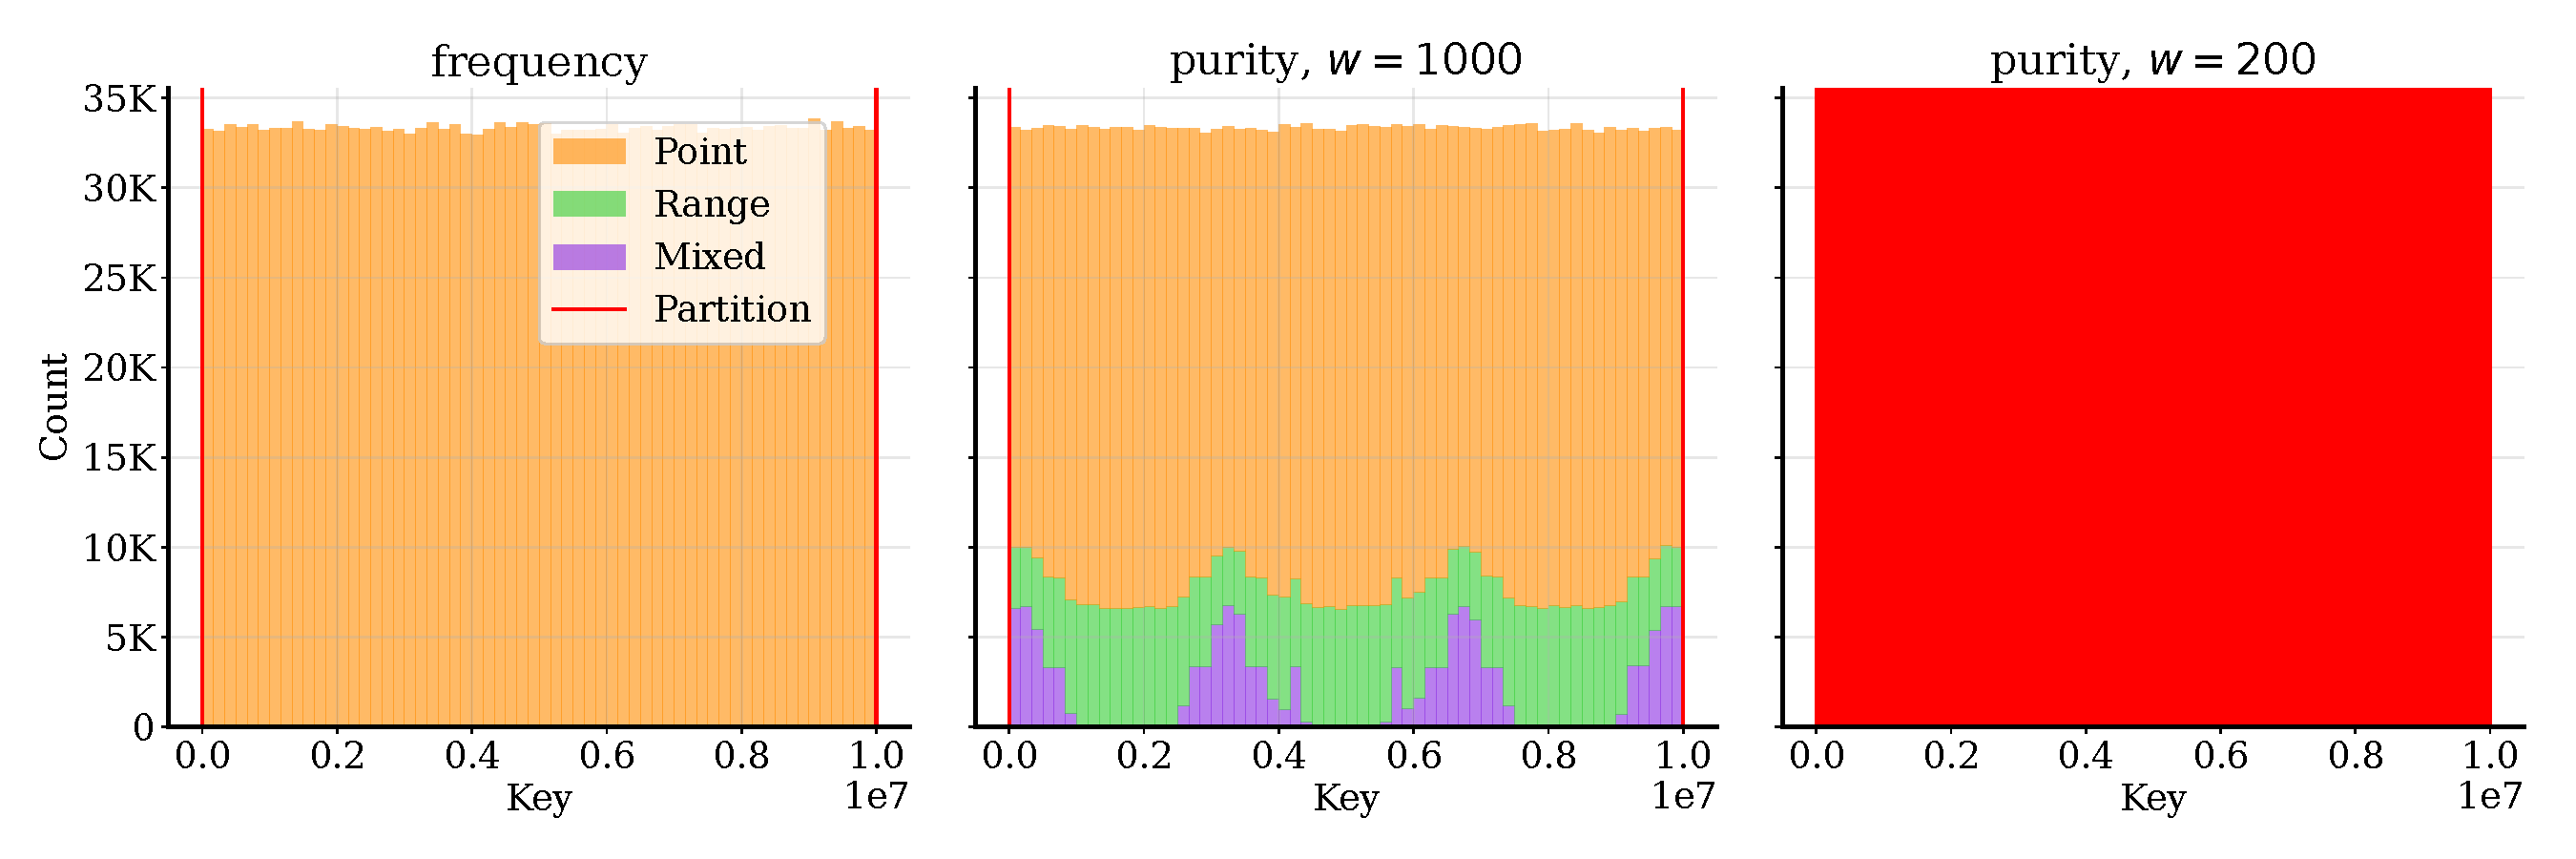
\includegraphics[width=\textwidth]{figures/exp3_query_dist.pdf}
    \caption[Worst case query distributions for partitioning]{Query distribution in the worst case for frequency partitioning}
    \label{fig:freqworst}
\end{figure}

The results of this experiment can be seen in \Cref{fig:freqworsttimes}. While our baseline B-tree index needs around 500 ns for one lookup, ART and PGM achieve significantly better lookup times below 200 ns. As mentioned before, uniform dense data is almost the best case for these index structures. Our index performs significantly worse than these two but is still competitive with the B-tree. We also notice that one single partition is not really the worst case, as our index needs around 350 ns per query. The performance is worse when we have many small partitions, i.e.~for the purity algorithm with a small window size. Here our index needs approximately the same time as the B-tree.

Returning to our initial question, we can conclude that in the worst case, the performance of our index degrades significantly. While the wrong choice of hyperparameters can lead to only one single partition or a multitude of small partitions, we found that our index with one single partition still performs better than the index with lots of partitions. Although the results suggest that our index stays competitive with a B-tree, we need to consider the extra time the partitioning takes. Including this, we would rather choose a B-tree over our index when the lookup times are only similar. We need to note, however that we described a possible optimization depending on the frequency information in \Cref{sec:leaftransform}, which, as mentioned, was not implemented yet. Therefore, the results here might be improvable if this or a comparable technique were realized. 


\begin{figure}
    \centering
    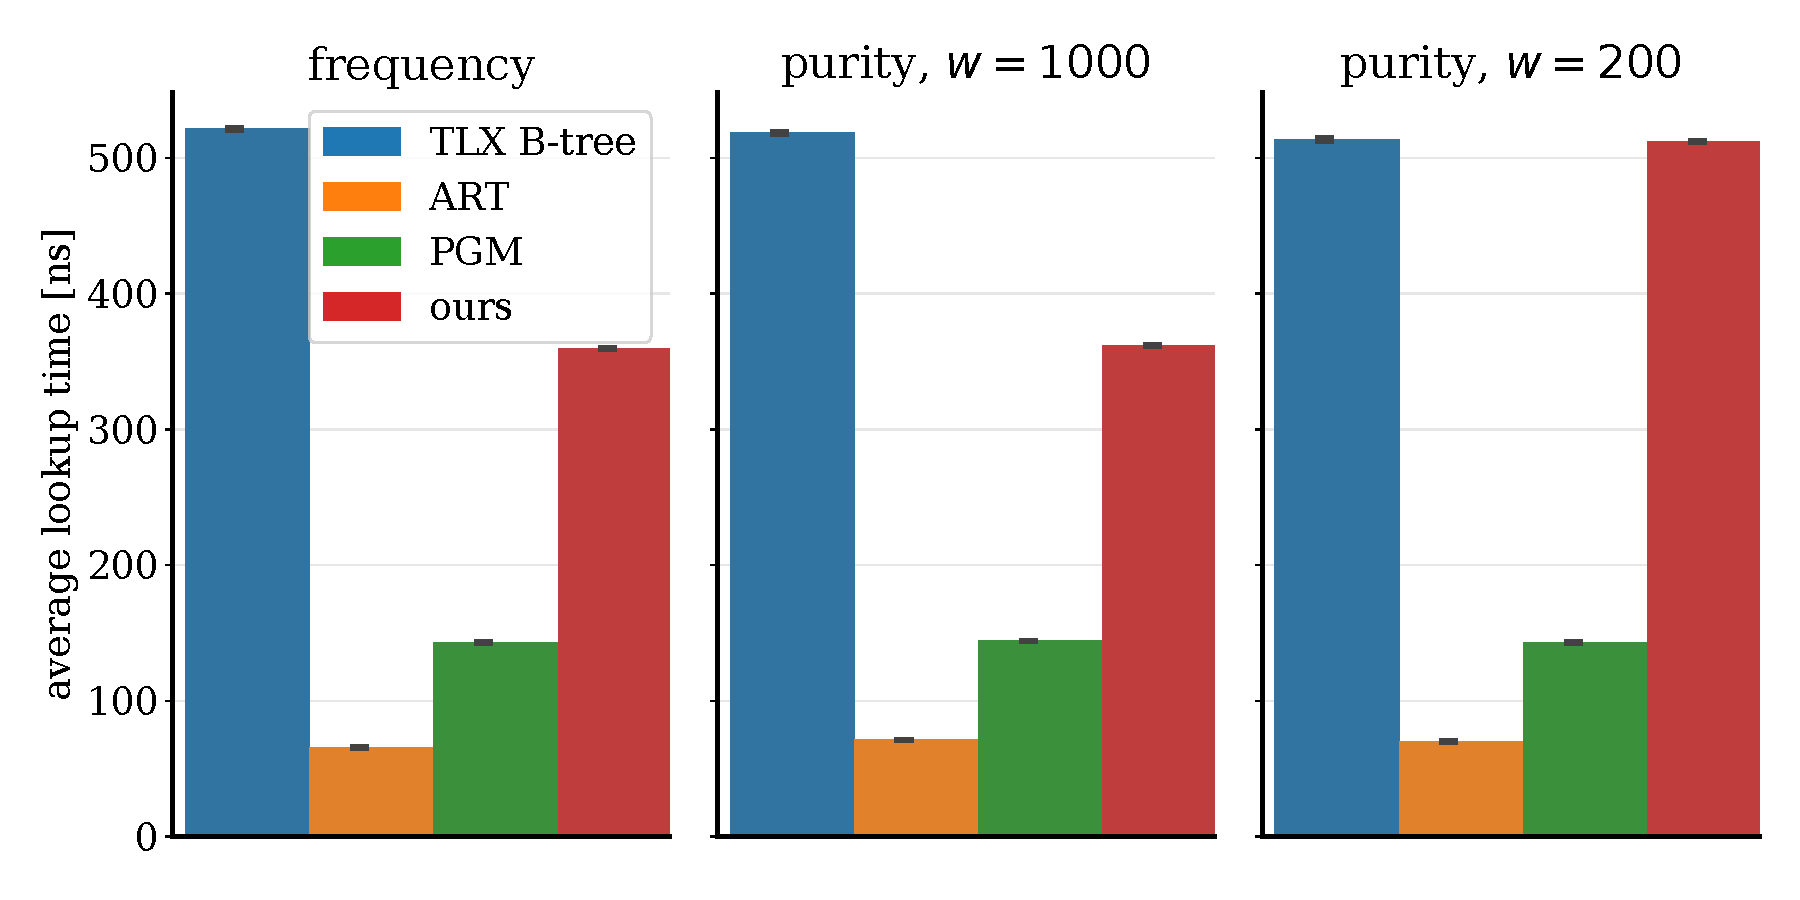
\includegraphics[width=0.9\textwidth]{figures/exp3_poc_times.pdf}
    \caption[Worst case lookup performance for partitioning]{Average query lookup time on a uniform, dense data using worst-case workloads}
    \label{fig:freqworsttimes}
\end{figure}

\subsection{Frequency partitioning over skewed distributions}
The next question that we considered was whether our index performed well under more realistic query distributions. According to \citeauthor{Anneser2022} \cite{Anneser2022}, common patterns in real-world workloads often include skewness. This experiment, therefore, answers the question:

\begin{center}
    \textit{Can our workload-based partitioning yield a comparable performance to the state-of-the-art under skewed workload conditions?}
\end{center}


\begin{figure}[!ht]
    \centering
    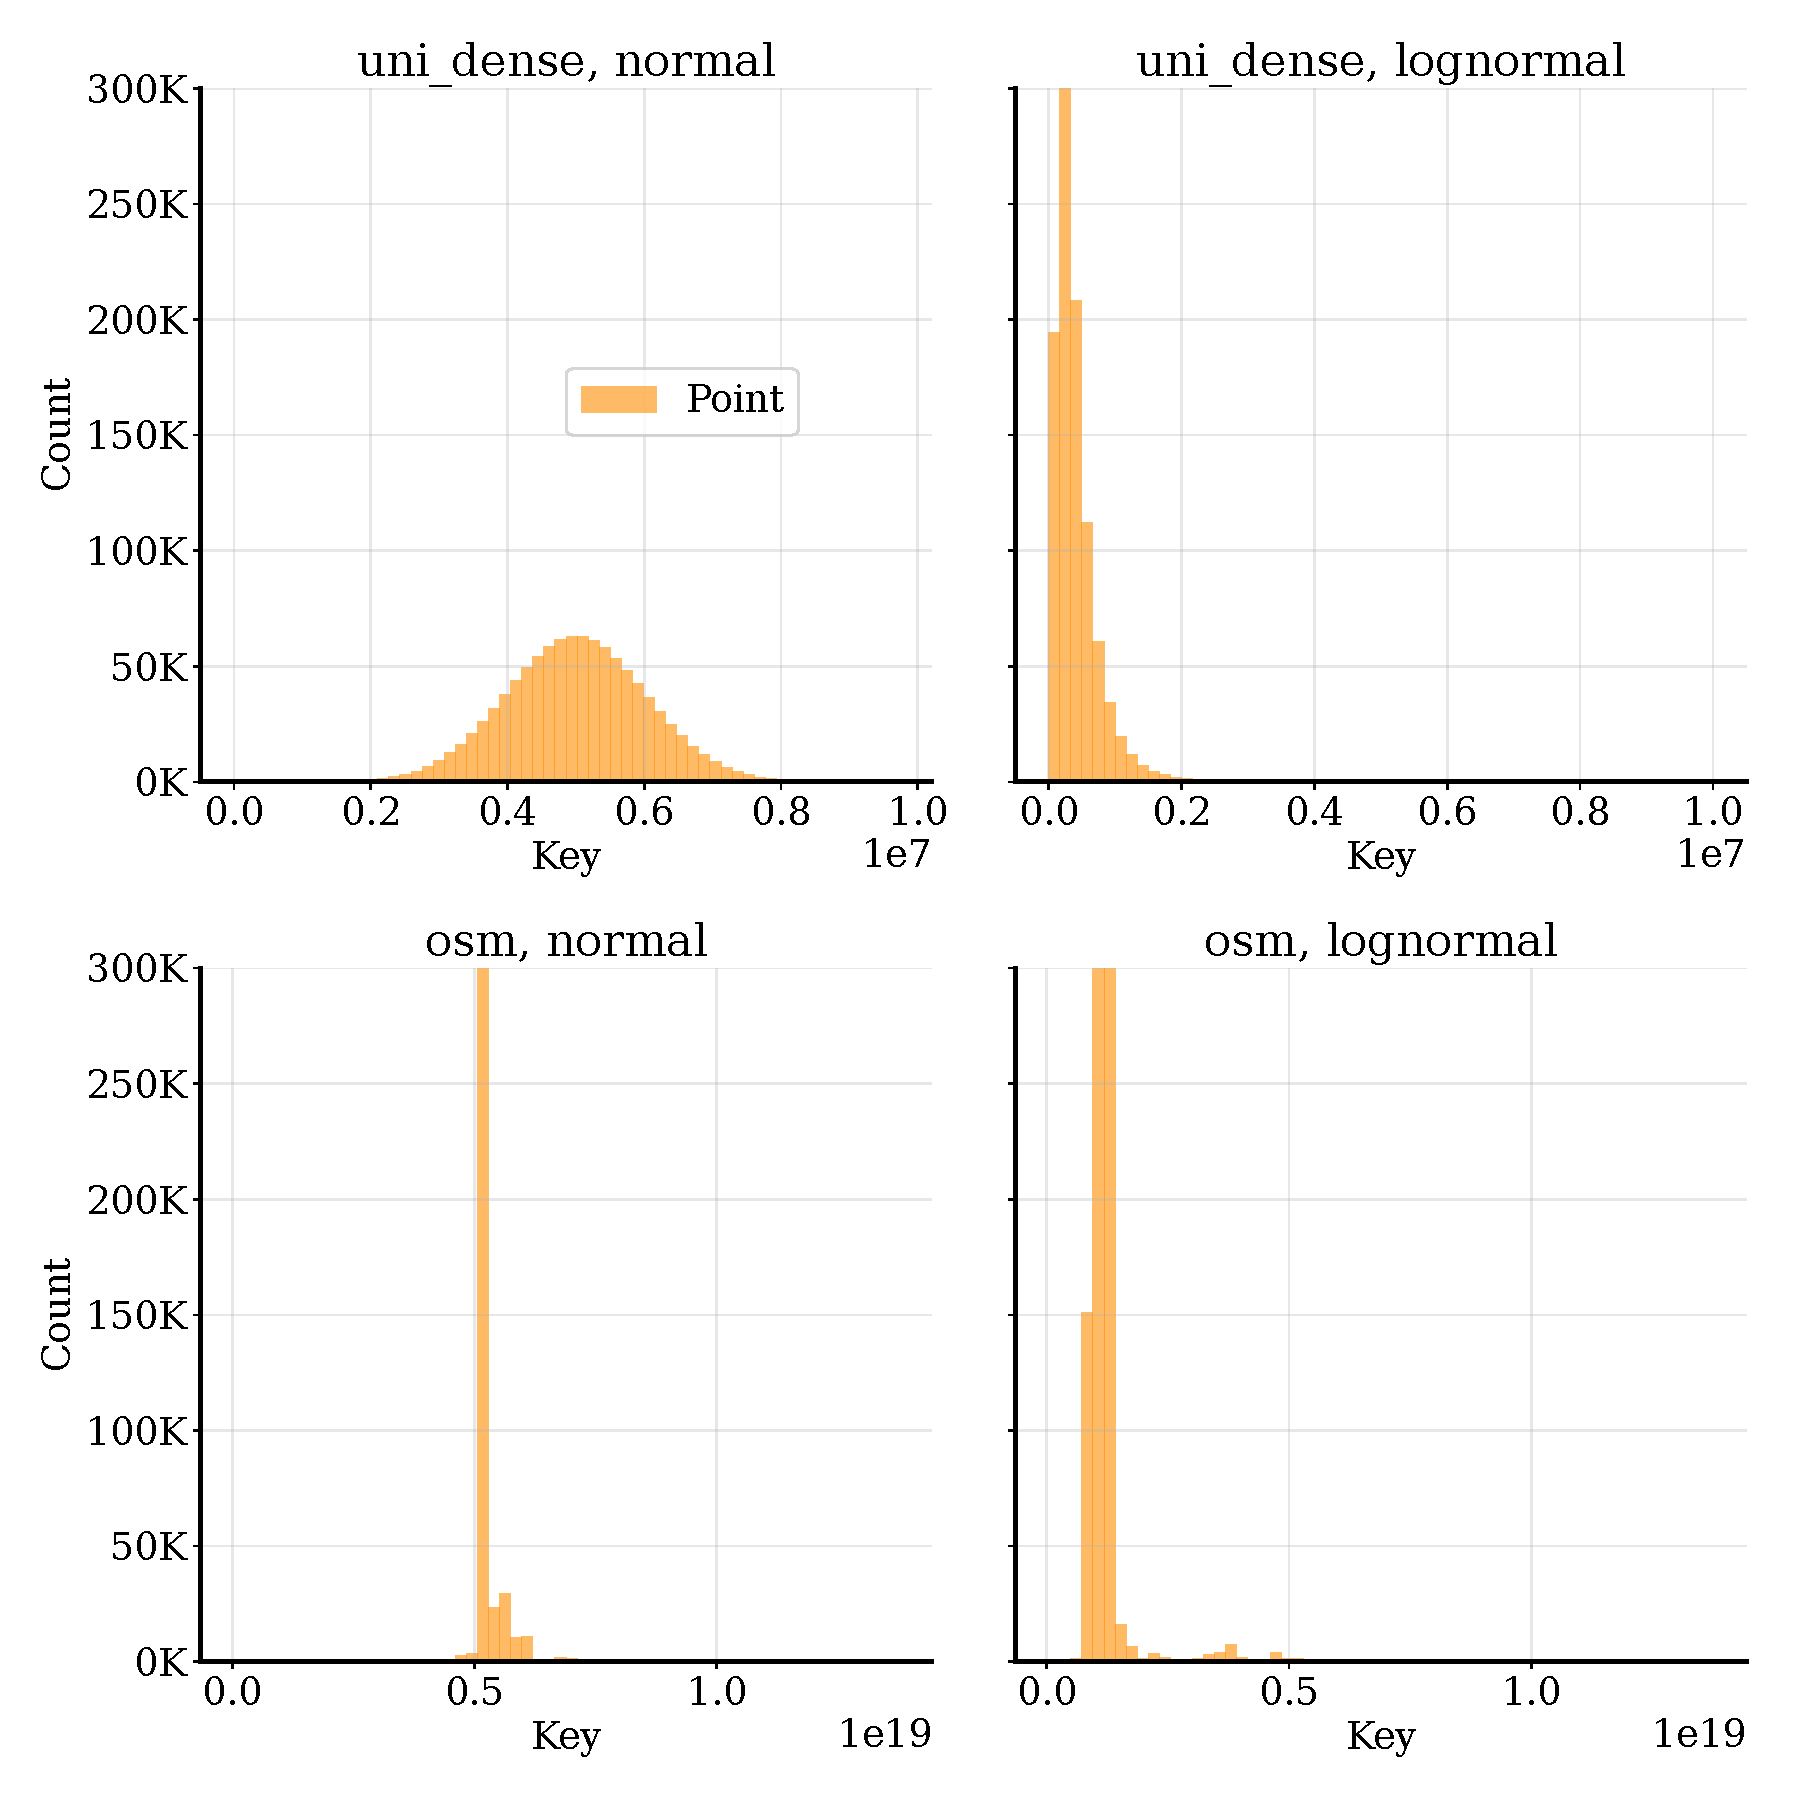
\includegraphics[width=0.9\textwidth]{figures/exp2_query_dist.pdf}
    \caption[uni and osm query distributions after normal and lognormal sampling]{Query distribution using normal and lognormal workloads on a uniform dense and the osm dataset}
    \label{fig:skeweddist}
\end{figure}

\noindent Similar to their workload selection, we also included a normal and lognormal workload to answer this question. As a third skewed workload, we included a gamma distribution. The parameters for the normal and lognormal distribution were selected according to \citeauthor{Anneser2022}. For the normal distribution, we choose $\mu = 0.5, \sigma = 0.03$, for the lognormal distribution, we choose $s = 0.7, \mu = 0, \sigma = 0.1$ and for the gamma distribution, we choose $a = 1.2, \mu = 0, \sigma = 0.1$. As the gamma distribution is very similar to the lognormal distribution with just slightly less skewness, we include all relevant plots in \Cref{app:skew}. We choose to evaluate the distributions on uniform, dense data and the real-world \verb|osm| dataset because it has different patterns across the dataset. The other real-world datasets mostly have only one significant distribution pattern, and as the partitioning algorithm takes quite some time to run, we decided not to investigate them further. For the same reason, we again decided to choose the reduced datasets with a size of 10 million. 

\Cref{fig:skeweddist} shows the query distribution of these workloads on the uniform dense and \verb|osm| dataset. For the \verb|osm| dataset, we can clearly see that the queries are mostly centered around the points where the dataset is especially concentrated. This relation is obvious when we look back at \Cref{fig:cdfs}. Because of the skewness, the lognormal distribution selects keys near the first jump in the CDF, whereas the normal distribution selects those near the second jump in the CDF. We tried to adjust the hyperparameter such that we do not fall into a case described in the previous experiment, namely a single large partition or thousands of small ones. In the end, we landed at window size $w = 200$ and $\delta = 0.15$, resulting in 60 to 116 partitions depending on the dataset and workload. Even small changes in both parameters resulted in situations like the worst cases from above. Because we do not have an automatic way to choose the parameters, we settled for the ones we found well aware that there might be a better configuration that we just did not try out.

\begin{figure}[!ht]
    \centering
    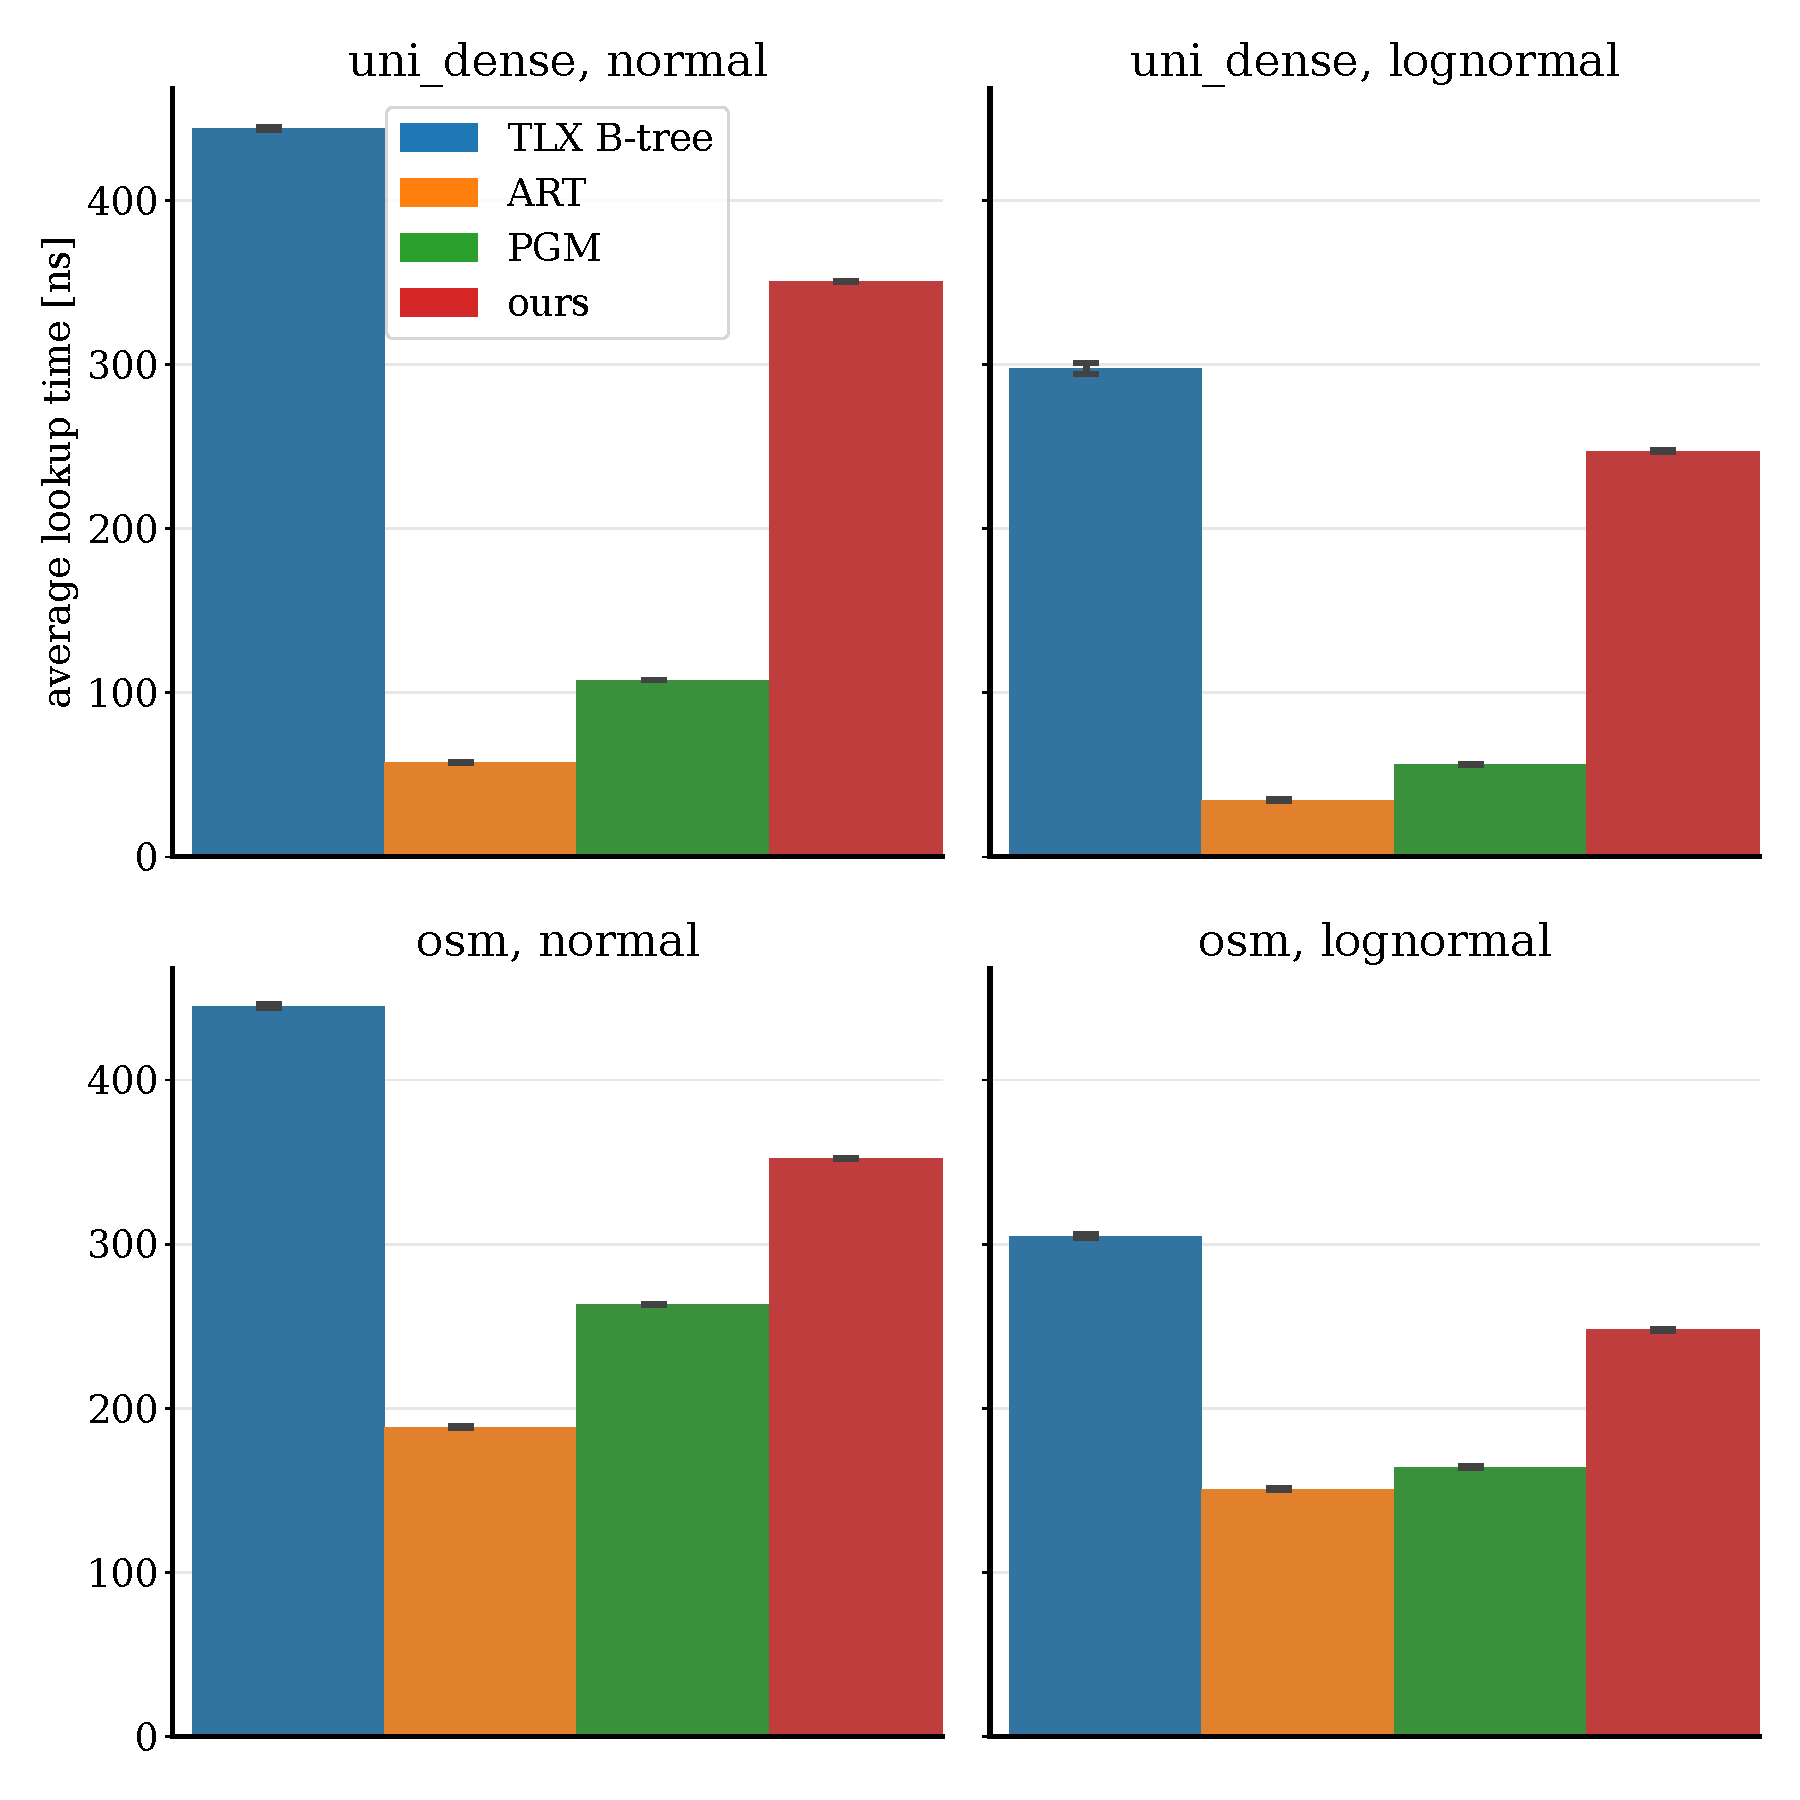
\includegraphics[width=0.9\textwidth]{figures/exp2_times.pdf}
    \caption[uni and osm lookup performance after normal and lognormal sampling]{Average query lookup time on uniform, dense data and the osm dataset using skewed workloads}
    \label{fig:skewedtimes}
\end{figure}


\Cref{fig:skewedtimes} shows the results of this experiment. We can directly see that there is a general trend across all scenarios, namely that the lognormal workload is faster to execute than the normal one. We can further observe that, especially for the uniform dense case, our index is significantly slower than ART and PGM, which take less than 100 ns. However, this difference is less significant for the osm dataset because ART and PGM need slightly more time per query. We can also observe that our performance is stable across the two different datasets, where we need around 350 ns for the normal workload and 250 ns for the lognormal workload.

Coming back to our question in the beginning, we need to state that our partitioning-based index is not competitive with the state-of-the-art index structures ART and PGM, at least when no optimization is performed based on the frequency. We also note that we can still outperform the B-tree, our weakest baseline.



\subsection{Influence of index misses}

\begin{minipage}{\textwidth}
As we have only sampled index-based until this point, the following question arises:

\begin{center}
    \textit{Does the number of queries requesting a key not in our index influence the performance of our index?}
\end{center}

\end{minipage}

\noindent To answer this question, we revisit the distributions from the previous experiment and see how our index performance changes when we do not completely sample index-based. To reiterate, index-based sampling means that we sample the indices of our underlying data and then convert these indices back to actual data points. This means that we will always sample a key that is present in our data. The second approach is sampling domain-based, meaning we directly select keys that fall in the range of our data points. For the sparse \verb|osm| dataset, this means that almost all keys that we sample domain-based will not be contained in the dataset itself, especially if we only use the downsampled \verb|osm| dataset with 10 million points. For our experiment, we chose to sample the \verb|osm| dataset with varying amounts of domain-based queries. We used uniform, normal and lognormal distributions with 0 \%, 20 \%, and 50 \% domain-based queries. We tried again to keep the number of partitions approximately equal across the different percentages, as we did not want to incur more costs by having to traverse more levels in our index. The configuration of hyperparameters for each combination of workload and percentage can be found in \Cref{tab:indexmisses}. As the query distributions on the \verb|osm| dataset are known from the previous experiment, we do not show them again here. The corresponding plots with small differences due to the new sampling method can be found in \Cref{app:misses}.

\begin{table}[ht]
\centering
\begin{tabular}{rrrrr}
\hline
distribution & percentage misses & $w$   & $\delta$ & partitions \\ \hline
uniform      & 20                & 200  & 0.12      & 29         \\
uniform      & 0                 & 200  & 0.13      & 21         \\
uniform      & 50                & 200  & 0.09      & 49         \\
normal       & 0                 & 500  & 0.15      & 85         \\
normal       & 20                & 200  & 0.15      & 83         \\
normal       & 50                & 200  & 0.15      & 148        \\
lognormal    & 0                 & 200  & 0.15      & 100        \\
lognormal    & 20                & 200  & 0.15      & 133        \\
lognormal    & 50                & 200  & 0.12      & 168        \\ \hline
\end{tabular}
\caption{Hyperparameter configuration depending on the workload distribution and the percentage of index misses/domain-based queries}
\label{tab:indexmisses}
\end{table}

\Cref{fig:exp4times} shows the results of this experiment. The first thing we observe is that the general trend from the previous experiment is also present here: the lognormal workload requires less time than the normal one. Another trend is that the more domain-based queries we have, the less time per query is required by all index structures. For the normal and lognormal workload distributions, there is almost no decrease in lookup time when going from 0 \% to 20 \%, which is very similar to all other indexes. The next step from 20 \% to 50 \% is connected to a decrease by 40 to 50 ns, which also happens for the other indexes. Only for the uniform sampling do we see a decrease of 100 ns when going from 20 \% to 50 \%. ART and PGM only decrease by approximately 40 ns in comparison. On the other hand, the B-tree also has a relatively large reduction of around 80 ns.

To summarize, we can say that the number of domain-based queries and, therefore, on our sparse dataset, the number of index misses impacts the average lookup time. An increase in this number for all indexes results in a decrease in the average query lookup time. Notably, our index does not seem to be an outlier to this general trend, the decrease we observe is always very similar to one of the other indexes.

\begin{figure}
    \centering
    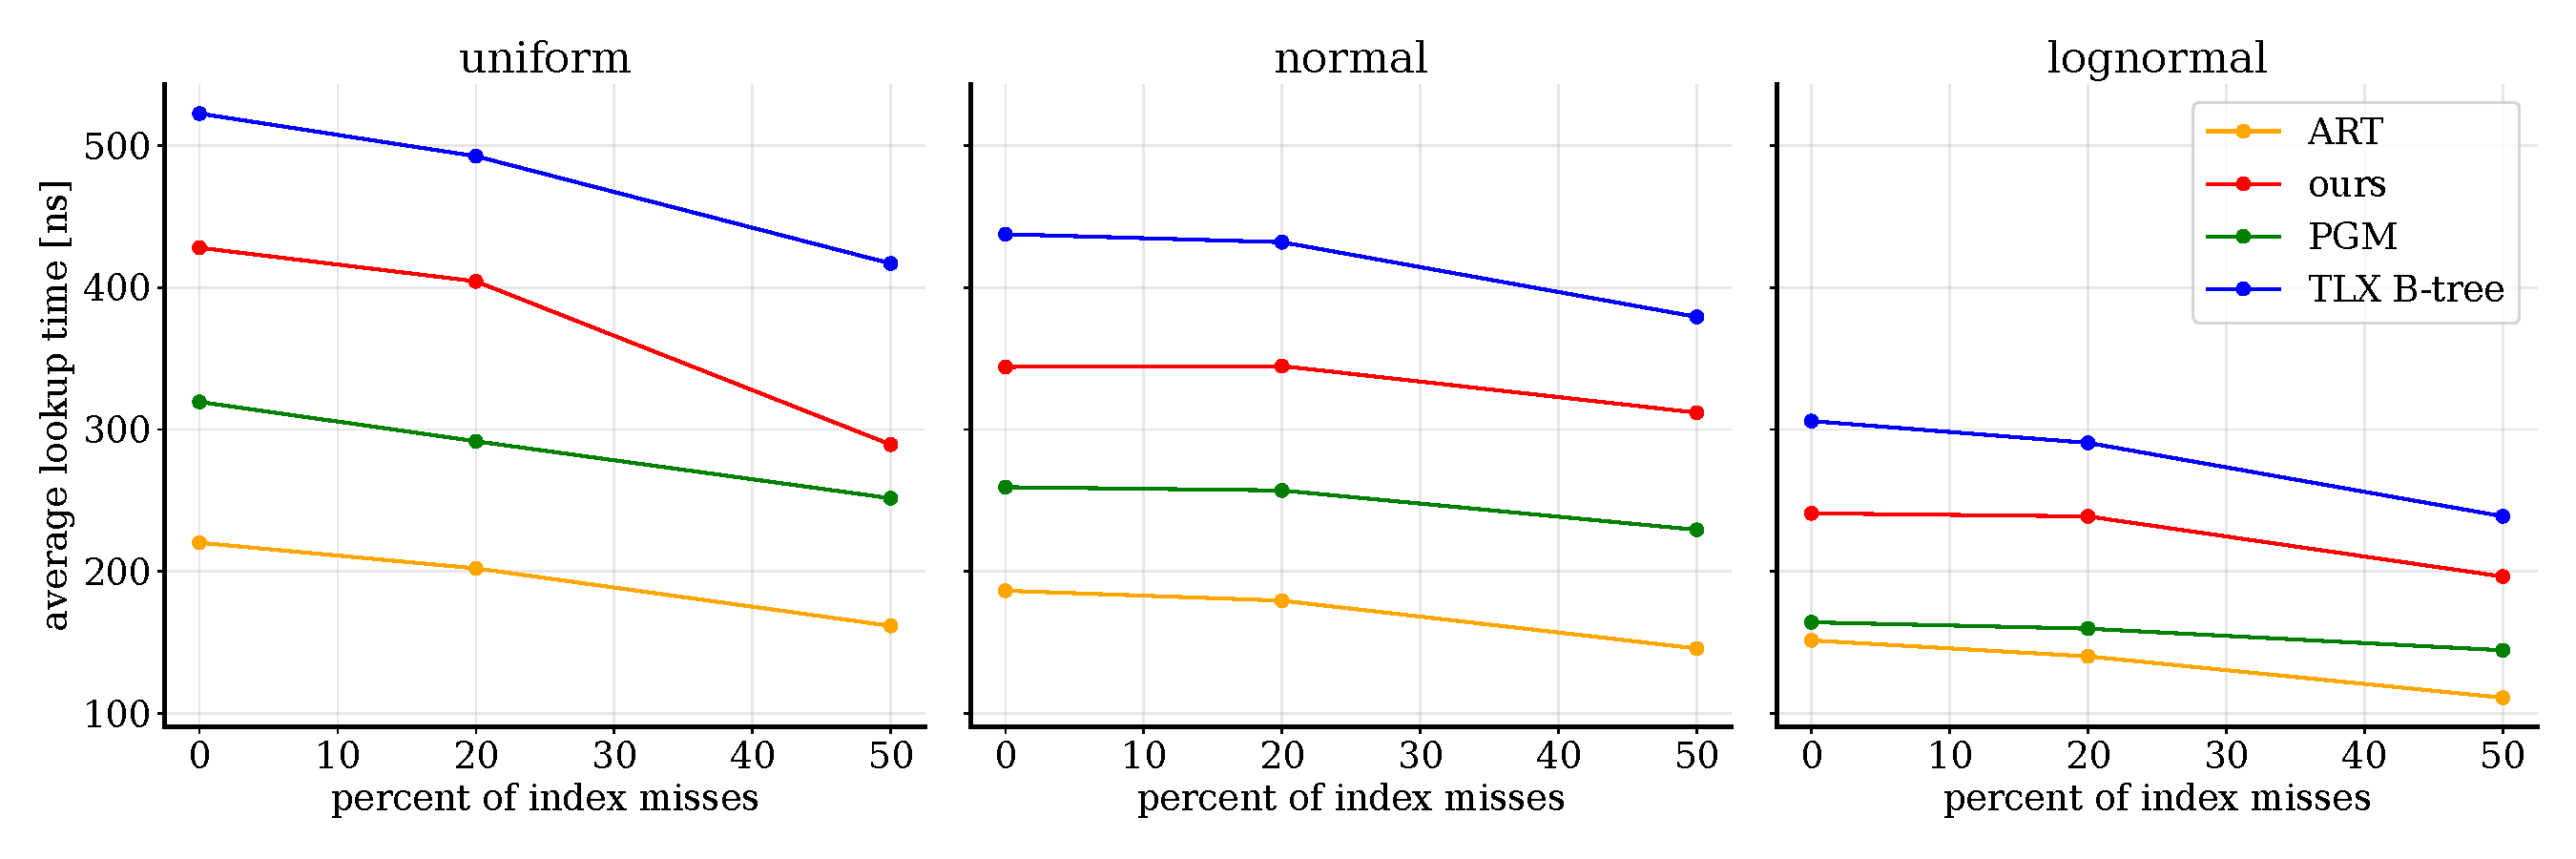
\includegraphics[width=\textwidth]{figures/exp4_times.pdf}
    \caption[osm lookup performance after sampling with index misses]{Average query lookup time on the osm dataset, depending on the percentage of index misses}
    \label{fig:exp4times}
\end{figure}

\subsection{Discussion}
At last, we want to address some points that influenced our research when answering our questions. First of all, we had the goal of covering a wide variety of workloads which we tried to do with customized scenarios. However, as we mentioned before, it was very time-consuming to calculate and manually inspect the partitions in relation to the workload distribution. As we do not have a mechanism to adjust our hyperparameters $w$ and $\delta$ automatically, we had to iterate over these values until we found a reasonable configuration. This excludes those configurations that produce way too many or one single partition, as we have seen in our second experiment. Because this iteration includes the partitioning step that takes several minutes to complete, we focused on rather simple workloads with a reduced dataset size. We are well aware that reducing the real-world datasets from 200 million keys to 10 million is a step that threatens the generalizability of the results we found. 

Another point we would like to mention is the structure of our index. While the main goal of this thesis was to develop the algorithms for partitioning, we naturally needed a way to evaluate these. Apart from the visual inspection of created partitions, this was done using the indexing framework introduced in \cite{Dittrich2021}. While we managed to incorporate the purity properties into the index by changing the leaf data structures, we did not have enough time to also do this in the way it was described in \Cref{sec:leaftransform}. This is mainly due to the initial approach we targeted, namely moving leaves higher up in the index after it was created. This was not as straightforward as we initially expected because moving leaf nodes could result in necessary changes to the whole index. It might not be possible to just add a pointer to the child in an inner node one level higher up because all inner nodes operate at maximum capacity. In this case, we would need to split one inner node, rearrange the child nodes and add the new nodes to their respective parent nodes. If their parents also operated at maximum capacity, they would again need to split, which in the worst case leads to a cascade of changes throughout the index. However, for our purposes, we could directly rearrange leaves at the construction time of the index, which is the easier approach. An implementation there can be realized much quicker, but because we were too invested in the more complex approach, we did not think of the easier solution in time to incorporate it into our experiments. Also, because the frequency algorithm was the more sophisticated one, we used more experiments to evaluate it, but in the end, the results suffer from the fact that the frequency information inside a partition is not structurally exploited by the index. We hope that a corresponding enhancement will result in a better performance. As of now, our index is essentially just a B-tree with variable length leaf nodes, which does not provide a competitive lookup performance apart from very specialized scenarios. 

